\documentclass[12pt,oneside,onecolumn]{book}      
%\usepackage[nottoc]{tocbibind}
\usepackage[spanish]{babel}
\usepackage[T1]{fontenc} %Paquetes de Fuentes que queramos usar
\usepackage[utf8]{inputenc}
\usepackage[spanish]{babel}
\usepackage{amsmath,amssymb,amsfonts}
\usepackage{fancyhdr}
\usepackage{graphicx} % Imagenes 
\usepackage{cite} 
\usepackage{hhline}
\usepackage{multicol}
\usepackage{longtable}
\usepackage{amssymb}
\usepackage{t1enc}
\usepackage[letterpaper, left=3cm, right=2cm, top=2cm, bottom=2cm]{geometry} 
\usepackage{amsmath}
\usepackage{color}
%\usepackage[export]{adjustbox}
\usepackage{pdfpages}
\usepackage{subcaption}
\usepackage{hyperref}
\usepackage{listings}
\usepackage{float}
\usepackage{textcomp}
\usepackage{appendix}



\AtBeginDocument{%
  \renewcommand\tablename{Tabla}
  \renewcommand{\bibname}{Referencias}
  \renewcommand{\contentsname}{Índice}
  \renewcommand{\listfigurename}{Índice de Figuras}
  \renewcommand{\listtablename}{Índice de Tablas}

}

% Redefinition of ToC command to get centered heading
\makeatletter
\renewcommand\tableofcontents{%
  \null\hfill\textbf{\Large\contentsname}\hfill\null\par
  \@mkboth{\MakeUppercase\contentsname}{\MakeUppercase\contentsname}%
  \@starttoc{toc}%
}
\makeatother
%Para encabezados y Pies de Pagina
\pagestyle{fancy}
   \lhead{}
    \chead{}
    \rhead{}
    \lfoot{}
    \cfoot{}
    \rfoot{\thepage}


\fancyhead[R]{}
    \renewcommand{\headrulewidth}{0pt}
%   \renewcommand{\footrulewidth}{0.4pt}


\fancypagestyle{plain}{%
    \renewcommand{\headrulewidth}{0pt}%
    \fancyhf{}%
    \fancyfoot[R]{\thepage}%
}

 \newtheorem{theorem}{Teorema}[chapter]
%\newtheorem{corollary}[theorem]{}
%\newtheorem{claim}{Claim}
\newtheorem{definition}{Definici\'on}[chapter]
\newtheorem{example}{Ejemplo}[chapter]
\newtheorem{proposition}{Proposici\'on}[chapter]
\newtheorem{myclaim}{Claim}[chapter]

\newcommand{\rand}{\stackrel{\$}\leftarrow}



%opening
%\title{}
%\author{}

\begin{document}

\begin{titlepage}
	\parbox{2cm}{
	\begin{picture}(18,4)
	    \put(-21,240){
\includegraphics[width=2cm,height=3cm]{./images/IPN.jpg}}
	    \put(0,-280){
\includegraphics[width=0.5cm,height=18.3cm]{./images/lineaAzul.jpg}}
	    \put(-37,-335){
\includegraphics[width=3cm,height=3cm]{./images/ESCOM.jpg}}
	    \end{picture}}
	\parbox{14cm}{\vspace{1cm} 
	    
	    {\fontsize{19}{30} \textbf{  INSTITUTO POLIT\'ECNICO NACIONAL}}
	    \begin{center}
	    {\fontsize{16}{20} \textbf{Escuela Superior de C\'omputo}}\vspace{1cm}\\
	    {\fontsize{18}{20} \textbf{ESCOM}}\vspace{2cm}\\
	    
	    {\fontsize{14}{20} \textit{Trabajo Terminal}}\vspace{1cm}\\
	    {\fontsize{16}{20} \textbf{``Protocolo criptográfico para el almacenamiento sin duplicados en la nube, resistente a ataques por fuerza bruta.''}}\vspace{1cm}\\
	    {\fontsize{14}{20} \textit{2016-B045}}\vspace{1cm}\\
	    {\fontsize{14}{20} \textit{Presentan}}\\
	    {\fontsize{14}{20} \textbf{Eder Jonathan Aguirre Cruz \\ Diana Leslie González Olivier \\ Jhonatan Saulés Cortés }}\vspace{2.5cm}\\
	    {\fontsize{14}{20} \textit{Directora}}\\
	    {\fontsize{14}{20} \textbf{Dra. Sandra D\'\i az Santiago}}\vspace{4.5cm}\\
	    \end{center}

	    \hfill  \fontsize{14}{20} \textbf{Mayo 2017}
	    
	}
\end{titlepage}

\frontmatter

\tableofcontents
\listoffigures

\listoftables
\mainmatter
%\chapter{Introducci\'on} % (fold)
%\label{cha:introduccion}
%\addcontentsline{toc}{chapter}{Introducción}



En el nuevo ambiente de las tecnologías de la información el almacenamiento de archivos puede ser realizado mediante modelos basados en el cómputo nube. \\
El cómputo nube es un término utilizado para nombrar así a la provisión de servicios de almacenamiento a través de Internet que ha sido utilizado para facilitar el cambio de los modelos de negocios, agilizar procesos y reducir costos de operación ~\cite{Nubei}. \\  

Uno de los mayores beneficios que ofrece este servicio es la virtualización de los centros de datos, que pueden operar de manera automatizada, sin necesidad de la presencia de una persona física y pueden ser gestionados en cualquier momento. De acuerdo con un estudio realizado por la consultora Market Research Media, estima que el cómputo nube generará \$270,000 millones de dólares en 2020, por lo que empresas como Google, Amazon, IBM, Oracle y Apple han adoptado este sistema como parte del servicio brindado a sus consumidores, por ejemplo, Google Drive o iCloud, a través de los cuales, con sólo estar conectados a Internet, los usuarios tienen la posibilidad de utilizarlos ~\cite{Nubecomp}. \\ 

Sin embargo, este servicio también presenta algunas desventajas que tal vez nosotros como usuarios no podemos percibir tan fácilmente. Una de ellas es que al almacenar un archivo en realidad no sabemos quién o qué entidades tienen acceso a él. Éste tema se está volviendo cada vez más preocupante sobre todo para instituciones o empresas que cuentan con información confidencial y también debido a diversos ataques por adversarios. \\

Es por eso que se ha optado por la opción del uso de la criptografía, la cual es una ciencia que se encarga de ocultar información, de tal forma que cualquier otra persona no pueda acceder al contenido. \\
%del estudio de técnicas para transformar la información a una forma que no pueda entenderse a simple vista; sin embargo, su objetivo no es sólo mantener los datos secretos, sino también protegerlos contra posibles modificaciones o manipulaciones y comprobar la fuente de los mismos  ~\cite{fundamentos}. \\

Ahora bien, la información que circula en dispositivos electrónicos es mayor a la memoria disponible que ofrecen estos, a medida que el volumen de información aumenta, también lo hace la demanda para los servicios de almacenamiento en la nube. Entonces los usuarios tienden a creer que el espacio en la nube es ilimitado y comienzan a guardar grandes cantidades de archivos, por lo cual nos enfrentamos al problema de la duplicación de archivos. \\ 

Es por ello que en el presente documento se propone una solución a estos problemas. Se trata de un protocolo criptográfico que nos brinda la confidencialidad de los archivos a la vez que nos ayuda a evitar la duplicación de los mismos. \\





%\section{Contexto}

%La criptografía es una ciencia que estudia técnicas matemáticas relacionadas con aspectos de seguridad de la información como confidencialidad, integridad de la información, entidades de autenticación y la autenticación de origen de datos entre otras. Esta ciencia tiene como principal objetivo el establecer la comunicación ya sea entre dos personas o dos entidades que requieren compartir información por un canal inseguro el cuál está propenso a un ataque para la manipulación o robo de esta información que viaja en el canal. Es por ello que la criptografía provee de protocolos, algoritmos y demás herramientas que ofrecen una solución para disminuir los ataques no deseados a la información que se requiera compartir de forma segura ~\cite{menezes}.
%\\ \\
%Estos protocolos, algoritmos y técnicas de la criptografía pueden ser utilizadas en distintas áreas de investigación o desarrollo, entre ellas esta el \textbf{Cómputo Nube}. La aplicación de la criptografía en los modelos computacionales basados en el cómputo nube tiene como objetivo proporcionar los algoritmos y protocolos criptográficos que den solución a los problemas en el crecimiento de los grandes volúmenes de información que hoy en día se tienen registro en el servicio de almacenamiento en línea \textbf{(Nube)}, basándose en la eliminación de la información que se encuentre con una copia exacta en la nube. Por ejemplo: 
%\\ \\
%El usuario registrado e identificado dentro de la nube como \textit{Usuario A}, el día de hoy desea almacenar un archivo \textbf{Archivo F} que corresponde a la especificación de los requisitos para la obtención de una beca escolar. Este usuario para no extraviar o modificar el archivo lo almacena en la nube y ahí queda disponible para cuando el lo solicite. Ahora este usuario comparte este archivo mediante un dispositivo \textit{USB} a su amigo ya que este también desea conocer los requisitos para solicitar una beca escolar, este amigo el cuál es otro usuario registrado e identificado dentro de la nube como \textit{Usuario B} también quiere almacenar este archivo \textbf{Archivo F} en la nube, ya que requiere utilizar el espacio de memoria en su dispositivo \textit{USB} para otras actividades y no desea perder los requisitos para la solicitud de su beca escolar. \\
%Ahora en la nube se encuentran almacenados 2 copias del \textbf{Archivo F} por dos diferenes usuarios identificados como  \textit{Usuario A} y \textit{Usuario B}, ambos almacenaron el mismo archivo en el mismo lugar, sin darse cuenta que ahora este archivo se encuentra duplicado en la nube. 



%Según un estudio realizado por Mundo de la informática (una revista mundial reconocida por su enfoque a las tecnologías de la información y comunicación) a empresas de tecnologías de la información, aseguran que el 42\% de estas empresas de TI están planeando aumentar el gasto en cómputo nube, siendo el crecimiento mayor en las empresas con más de 1000 empleados (52\%). Las 5 áreas de mayor crecimiento se ilustran en la figura ~\ref{fig:1-1-1}

%\begin{figure}[H]
%\centering
%	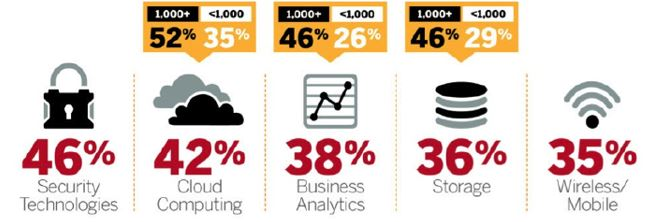
\includegraphics[width=15cm, height=5cm]{./images/aumentoCloudComputing.jpg}
%	\caption{Aumento del gasto por las empresas en cómputo nube}
%	\label{fig:1-1-1}
%\end{figure}


%El cómputo nube es un término general utilizado para nombrar así a la provisión de servicios de almacenamiento a través de internet que ha sido utilizado para facilitar el cambio de los modelos de negocios, agilizar procesos y reducir los costos de operación en las grandes empresas u organizaciones. 

%De acuerdo con un estudio realizado por la consultora Medios de investigación de mercado \textit{(Market Research Media)}, el cómputo nube generará \$270,000 millones de dólares en 2020, por lo que empresas como Google, Amazon, IBM, Oracle y Apple han adoptado este sistema como parte del servicio brindado a sus consumidores, por ejemplo Google Drive o iCloud, a través de los cuales, con sólo estar conectados a Internet, los usuarios tienen la posibilidad de utilizarlos ~\cite{Nubecomp}. \\ \\ 

%Básicamente el almacenamiento en la nube se caracteriza por 5 puntos esenciales que son: 
%	\begin{itemize}
%		\item \textbf{Autoservicio on-demand o pago por evento}  
%		\item \textbf{Acceso ubicuo a la red (uso de los servicios cuando sea y donde sea)}  
%		\item \textbf{Fondo común de recursos} 
%		\item \textbf{Rápida elasticidad} 
 %		\item \textbf{Servicio medido}  ~\cite{Compnube}.
 %\end{itemize}



\section{Planteamiento del problema.}
Hoy en día millones de personas en el mundo tienen la facilidad de acceder a un dispositivo electrónico que les permite manipular información o almacenarla ya sea en un dispositivo físico o en la nube.
Debido a los limitados recursos financieros y altos gastos de almacenamiento de datos electrónicos, los usuarios prefieren almacenar sus datos en los entornos de nube provocando enormes demandas a las compañías que ofrecen este servicio. El incremento en el uso de estos servicios implica que los sistemas de almacenamiento tengan más capacidad y puedan cubrir la alta demanda que se presenta en el mercado ~\cite{Keelveedhi}. \\

%Ahora bien, la información que circula en dispositivos electrónicos es mayor a la memoria disponible que ofrecen estos, a medida que el volumen de información aumenta, también lo hace la demanda para los servicios de almacenamiento en línea ~\cite{Bellare}. Un gran incremento en el uso de estos servicios implica tener más infraestructura y personal para que los sistemas de almacenamiento tengan más capacidad y puedan cubrir la demanda que se presenta en el mercado. Si bien el almacenamiento logró dar buenos resultados al cliente en sus primeras etapas, ahora la preocupación por el incremento de infraestructura para seguir dando esos resultados se ha incrementado considerablemente  ~\cite{Keelveedhi}.
%\\ 

Para entender un poco más acerca de la problemática a la que se enfrenta el almacenamiento en la nube, mostramos el siguiente estudio realizado por EFE/Cisco: \\ 

EFE/Cisco realizó una estimación en el año 2014 en su cuarto informe anual Índice Global sobre la nube (2013-2018), donde podemos observar en la figura ~\ref{fig:1-2-1} como el almacenamiento ha ido incrementado y seguirá incrementado \\

\begin{figure}[H]
\centering
	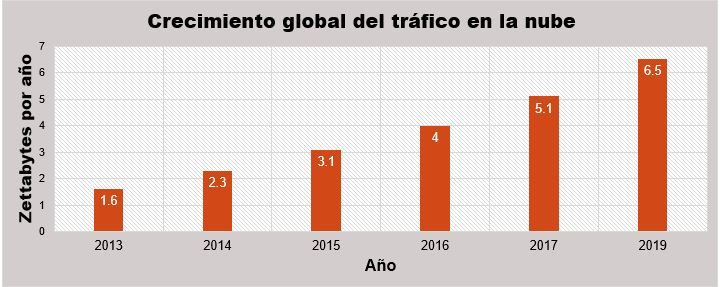
\includegraphics[width=13cm, height=5cm]{./images/crecimientoNube.jpg}
	\caption{Crecimiento global del tráfico en la nube}
	\label{fig:1-2-1}
\end{figure}

Una de las principales razones del incremento en el tamaño en la estructura de almacenamiento de servicios en línea es la duplicación de archivos, existen muchas copias en la nube de un mismo archivo que se encuentra presente en diferentes cuentas de usuarios. Un ejemplo: el usuario registrado e identificado dentro de la nube como \textit{Usuario A}, el día de hoy desea almacenar un archivo \textbf{Archivo F} que corresponde a la especificación de los requisitos para la obtención de una beca escolar. Este usuario para no extraviar o modificar el archivo lo almacena en la nube y ahí queda disponible para cuando él lo solicite. Ahora este usuario comparte este archivo mediante un dispositivo \textit{USB} a su amigo ya que este también desea conocer los requisitos para solicitar una beca escolar, este amigo el cuál es otro usuario registrado e identificado dentro de la nube como \textit{Usuario B} también quiere almacenar este archivo \textbf{Archivo F} en la nube, ya que requiere utilizar el espacio de memoria en su dispositivo \textit{USB} para otras actividades y no desea perder los requisitos para la solicitud de su beca escolar. \\

Ahora en la nube se encuentran almacenados 2 copias del \textbf{Archivo F} por dos diferentes usuarios identificados como \textit{Usuario A} y \textit{Usuario B}, ambos almacenaron el mismo archivo en el mismo lugar, sin darse cuenta que ahora este archivo se encuentra duplicado en la nube. \\

Otro punto importante es la seguridad e integridad de la gran cantidad de información que se almacena en la nube. Este servicio de almacenamiento está sujeto a los ataques de adversarios que están interesados en el robo, manipulación o alteración de la información. Uno de los ataques que se han intentado realizar por dichos adversarios es el ataque por fuerza bruta, el cual es una forma de recuperar una clave probando todas las combinaciones posibles hasta encontrar aquella que permite el acceso al archivo. \\

Por un lado si tenemos la información en claro es relativamente fácil poder detectar que dos archivos son los mismos, ya que solo se compara bit a bit, pero si estos mismos archivos cada usuario cifra su archivo el resultado serian dos archivos diferentes por esto es que no es posible detectar archivos duplicados con este método. \\
 \\  \\



%\section{Justificación}

%En la actualidad millones de personas usan los servicios de almacenamiento que ofrece la nube, ya sean gratuitos o privados, este número de personas ha ido en un incremento exponencial lo cual hace que el espacio de almacenamiento disminuya, entonces ¿Cómo podría mitigar el problema de almacenamiento y tener privacidad de los datos al mismo tiempo.\\

%Usando la criptografía clásica para poder cifrar un archivo se utiliza una clave privada la cuál es distinta para cada usuario, cada vez que se cifra un archivo el resultado de este es diferente para cada intento. Por tanto no se puede evitar la duplicación de archivos utilizando este mecanismo de la criptografía y se deben implementar soluciones más robustas.

%Una solución para tener privacidad y evitar duplicación la proporcionó John R. Douceur, la cual dice que teniendo a M que será el contenido de un archivo de aquí en adelante denominado el mensaje, el cliente primero calcula una clave K ← H(M) mediante la aplicación de una función de hash criptográfica H al mensaje y luego calcula el texto cifrado C ← E(K,M) a través de un esquema de cifrado simétrico determinista. El derivado del mensaje K se almacena por separado cifrándolo con una llave por cliente. Un segundo cliente B cifra el mismo archivo M que producirá el mismo C, evitando la duplicación ~\cite{donceur}. \\

%En el artículo publicado por Mihir Bellare, Sriram Keelveedhi, Thomas Ristenpart, nombrado “DupLESS: Server-Aided Encryption for Deduplicated Storage” ~\cite{Bellare}, se observó que uno de los principales problemas al que nos enfrentamos es que el esquema de cifrado solo es seguro cuando el espacio de mensajes es demasiado grande, por lo tanto agentes externos pueden provocar agravios a la integridad de la información de los usuarios.

%Si bien esta solución se ocupa de la duplicación de archivos deja muy vulnerable el aspecto de la privacidad, ya que ante un espacio de mensajes pequeño las amenazas del adversario son demasiadas. Si se tuvieran como ejemplo 1000 mensajes, para el adversario sería muy fácil intentar encontrar la clave, probando las 1000 claves posibles generadas con la función hash, hasta descifrar el archivo, por lo tanto se comprueba que un espacio de 1000 mensajes sigue siendo pequeño.

%Es por ello que este trabajo terminal tiene como principal meta atacar esta problemática de privacidad, proponiendo una arquitectura del sistema que a través de un servidor de llaves se generaran llaves de acuerdo al contenido del archivo, para con esta se pueda cifrar y luego almacenar en la nube donde se eludirá la duplicación de archivos. 



\section{Propuesta de solución. }

Como se mencionó anteriormente encontramos dos principales problemas, uno es la confidencialidad de los archivos cuando se almacenan en la nube y el otro es la cantidad de archivos duplicados en la misma. \\

Para combatir el problema de la confidencialidad, proponemos el uso de la criptografía, a cada usuario se le proporcionará una llave con la que puede cifrar y descifrar archivos, pero no podemos usar criptografía de manera tan simple ya que si dos usuarios cifran el mismo archivo daría como resultado dos archivos cifrados distintos, entonces al hacer la comparación de ambos archivos no habría forma de atacar el problema de la duplicación de archivos. Así que nos encontramos con otro problema, pues evitamos que los archivos estén expuestos a adversarios, pero seguimos con el problema de archivos duplicados.\\

 Por lo tanto, nos basaremos en el protocolo denominado DupLESS ~\cite{Bellare} el cual combina varias herramientas criptográficas de tal forma que se pueda tener un control de las llaves relacionadas con los archivos y los usuarios sin comprometer el contenido e integridad de la información, de esta manera si dos usuarios quieren cifrar el mismo archivo obtendrán la misma llave. Por consiguiente, al cifrar los archivos obtendríamos como resultado el mismo archivo cifrado, esta vez al hacer la comparación se detectará la duplicación de archivos y únicamente se guardará una copia del archivo, ahorrando espacio de memoria y costos de infraestructura. \\

Como se observa en la siguiente figura ~\ref{fig:1-3-1} varios usuarios realizan peticiones para subir archivos, pero se puede notar que algunos son iguales, por lo que pasan por un proceso de eliminación de duplicados antes descrito y finalmente se almacena una copia de cada uno. \\




%La eliminación de duplicación de datos es una técnica que avanza favorablemente y da como resultado la disminución drástica de la cantidad de información duplicada en la nube, cuando esta se elimina del almacenamiento. En general, la eliminación de duplicados compara la información nueva que se requiere almacenar con la información que ya se tiene archivada y elimina las duplicaciones en la nube reduciendo la asignación de almacenamiento dentro de esta, esta disminución en la nube puede reducir las necesidades de almacenamiento en hasta un \textit{80\%} para archivos y copias de seguridad que los usuarios resguardan en la nube como se ilustra en la figura ~\ref{fig:1-3-1}. Las ventajas de no tener duplicados en la nube incluyen una mayor capacidad de almacenamiento y ahorro presupuestario, al igual que la minimización del ancho de banda para menos costosa y más rápida la repetición de la información fuera de la reserva simplificando y mejorando la gestión del almacenamiento de datos  ~\cite{rededup}. 

\begin{figure}[H]
\centering
	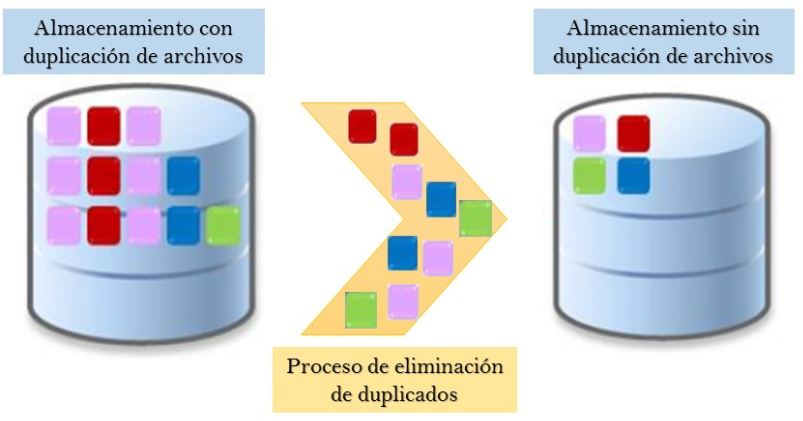
\includegraphics[width=10cm, height=5cm]{./images/Deduplicacion.jpg}
	\caption{Eliminación de Duplicados}
	\label{fig:1-3-1}
\end{figure}

%Una posible solución para la protección a los datos y eliminación de duplicaciones, es echar mano de la criptografía. Ciencia que se encarga del estudio de técnicas para transformar la información a una forma que no pueda entenderse a simple vista; sin embargo, el objetivo de la Criptografía no es sólo mantener los datos secretos, sino también protegerlos contra la modificación o manipulación y comprobar la fuente de los mismos ~\cite{fundamentos}. \\   \\
%Está ciencia que mantiene la información segura se encuentra dividida en dos grandes tipos: \textbf{Criptografía Simétrica} y \textbf{Criptografía Asimétrica}.  \\

%\textit{La criptografía simétrica} o también llamada criptografía de llave secreta, basa su seguridad en una sola llave que se comparte entre dos entidades que quieren compartir información, dicha llave es utilizada para cifrar un archivo al ser enviado a la otra entidad y este utilizará la misma llave para descifrarlo cuando lo reciba. \\
%\textit{La criptografía asimétrica} o criptografía de llave pública involucra el uso de un par de llaves para cada entidad que desea comunicarse, estas llaves llamadas pública y privada. Para que una entidad envíe un archivo a otra, necesita cifrar el archivo con la llave pública de esa entidad a la que se desea enviar, y cuando lo reciba esa entidad lo deberá descifrar con su llave privada o secreta. De esta manera se evita el compartir llaves para cifrar y descifrar como sucede en la criptografía simétrica y reduce los riesgos de un ataque de adversarios.  \\ \\


%El objetivo de esta propuesta de solución es almacenar más datos en menos espacio mediante el uso de la criptografía. Esta ciencia nos proveerá con sus herramientas para la creación de un llavero criptográfico, dicho llavero realizará una firma la cuál dará paso a la creación de una llave correspondiente a un archivo \textit{F} que se desee almacenar un usuario, si se llega a solicitar al llavero por un usuario diferente una nueva firma para la creación de una llave para el mismo archivo \textit{F}, esta llave será la misma, ya que el mecanismo de funcionamiento entre un usuario y este servidor está diseñado para que sea capaz de identificar el mismo archivo sin comprometer el contenido e integridad de este. Esta  llave va a lograr que cuando se cifre este archivo por \textit{n} cantidad de usuarios diferentes que lo poseen, dicho cifrado será igual para la \textit{n} cantidad de usuarios, permitiendo así que en la nube al subir estos cifrados se realice una comparación para que reconozca a quien pertenecen esos cifrados y sólo tenga almacenada una sola copia de este, ahorrando espacio de memoria y costos de infraestructura. 

%Puesto que ambas cuestiones, la eliminación de duplicados y la privacidad de la información, son importantes, se ha comenzado a
%proponer mecanismos que solucionen ambos problemas de manera conjunta, que son: Dupless ~\cite{Bellare}, ABS: the apportioned backup
%system. ~\cite{abs}, Flud Backup ~\cite{flud}, SIGOPS Oper. Syst. ~\cite{sigops}, TahoeFS ~\cite{tahoe}.


\section{Objetivos. } % (fold)

    \subsection{Objetivo General.} % (fold)
    Desarrollar un protocolo criptográfico para evitar la duplicación de archivos almacenados en la nube, garantizando la privacidad de los usuarios contra adversarios cuando el espacio de mensajes es pequeño, utilizando algoritmos criptográficos para su implementación. 
     
    \subsection{Objetivos Específicos.} % (fold)
	\begin{itemize}
		\item Evitar la duplicación de archivos que sean almacenados por los usuarios de la nube
		\item Proteger ante los adversarios la información de los usuarios de la nube
		\item Establecer un esquema de autenticación de usuarios 
		\item Reducir la pérdida y filtración de información de los usuarios de la nube
		\item Evitar los ataques por fuerza bruta al contenido de los archivos de usuarios en la nube. 
 	\end{itemize}

\section{Organización del documento. }

El presente documento que detalla todo el proceso de creación de este protocolo criptográfico está conformado por 6 diferentes capítulos los cuáles son: 

\begin{itemize}
	\item Capítulo 1 \textbf{Introducción} \\
                     En este capítulo se expone cuál es el contexto en el que este trabajo terminal se desarrollará, así mismo se describe cuá a sido la problemática detectada a partir del análisis del contexto en el cuál se desarrola la investigación y finalmente se muestran cuales son los objetivos tanto general como específicos de este trabajo terminal, es decir, cuál es la finalidad de éste protocolo criptográfico. 

	\item Capítulo 2 \textbf{Marco Teórico} \\
El contenido de este capítulo abordará temas estrechamente relacionados con la criptografía y la seguridad de la información. También, este capítulo contiene información acerca de los 2 tipos de criptografía que existen mencionando los diferentes esquemas de cifrado y los modos de operación que son utilizados por algunos de estos. De igual forma se describe con detalle los servicios que ofrece el cómputo nube. 

	\item Capítulo 3 \textbf{Estado del Arte} \\
	En dicho capítulo se encontrará plasmada una comparativa realizada entre sistemas o prototipos que tienen una similitud con el protocolo criptográfico que este trabajo terminal propone. Esta comparativa contendrá detalles técnicos enfocados a las herramientas criptográficas utilizadas en estos sistemas.

	\item Capítulo 4 \textbf{Protocolo Dupless} \\
            El capítulo 4 contiene a gran detalle el funcionamiento del protocolo criptográfico Dupless, dicho protocolo será la base de la investigación para el desarrollo de este trabajo terminal. 

	\item Capítulo 5 \textbf{Análisis} \\
	Como otro capítulo más de este documento se encuentra el análisis del protocolo criptográfico, el cuál se compone de la realización de un estudio de factibilidad y análisis de riesgos para la realización de este proyecto, asimismo se muestra cuál será la arquitectura de trabajo terminal, la descripción de todos los procesos que involucrán la creación de este protocolo, el modelo de entidades que comprende diagrama entidad relación y el diagrama de clases para su implementación. Al final de este capítulo se podran encontrar los requerimientos de este protocolo criptográfico tanto funcionales como no funcionales y las reglas de negocio que lo componen.

	\item Capítulo 6 \textbf{Diseño} \\
	El capítulo de diseño tiene como contenido la especificación de la plataforma del protocolo, es decir, la especificación de recursos necesarios para poder llevar a cabo su implementación con las herramientas necesarias, y también todos los casos de usos que involucran el funcionamiento de dicho protocolo.

\end{itemize}




    
\chapter{Preliminares. } % (fold)

El contenido de este capítulo abordará temas estrechamente relacionados con la criptografía, la seguridad de la información y las implicaciones que ésta podria traer si esta se encuentra corrompida por algun adversario. También, este capítulo contiene información acerca de los 2 tipos de criptografía que existen mencionando los diferentes esquemas de cifrado y los modos de operación que son utilizados por algunos de estos. De igual forma se describe con detalle los servicios que ofrece el cómputo nube, haciendo énfasis en un servicio en particular que es el de almacenamiento que se utilizará para la implementación de este protocolo criptogrráfico. 


\section{Definiciones. }
\textbf{Criptografía. }

La Criptografía es la ciencia que se encarga del estudio de técnicas matemáticas relacionadas con aspectos de seguridad  para transformar la información a una forma que no pueda entenderse a simple vista; sin embargo, el objetivo de la Criptografía no es sólo mantener los datos secretos, sino también protegerlos contra modificación y comprobar la fuente de los mismos. 


\textbf{Criptoanálisis. }
Es la ciencia que se ocupa del análisis de un texto cifrado para obtener la información original sin conocimiento de la clave secreta, esto es, de forma ilícita rompiendo así los procedimientos de cifrado establecidos por la Criptografía, por lo que se dice que Criptoanálisis y Criptografía son ciencias complementarias pero contrarias.
El criptoanálisis es el arte de descifrar comunicaciones cifradas sin conocer las llaves  ~\cite{cripto}.


\subsection{Servicios criptográficos. }
Los servicios criptográficos son aquellos que garantizan en un sistema de información la adquisición, almacenamiento, procesamiento y transmisión de la información y para lograrlo se valen de uno o más objetivos fundamentales. 

\textbf{Confidencialidad. }
Es un servicio utilizado para mantener el contenido de la información de todos, excepto los autorizados a tenerla. El secreto es un término sinónimo de confidencialidad y privacidad.
Hay numerosos enfoques para proporcionar confidencialidad, que van desde la protección física a los algoritmos matemáticos que hacen que los datos sean ininteligibles.

\textbf{Autenticación. }
Es un servicio relacionado con la identificación. Esta función se aplica tanto a las entidades como a la propia información. Dos partes que participan en una comunicación deben identificarse entre sí. La información entregada a través de un canal debe ser autenticada en cuanto al origen, fecha de origen, contenido de los datos, tiempo enviado, etc. Por estas razones este aspecto de la criptografía suele subdividirse en dos clases principales: autenticación de entidad y autenticación de origen de datos. La autenticación de origen de datos proporciona implícitamente la integridad de los datos (si se modifica un mensaje, la fuente ha cambiado).

\textbf{Integridad. }
Es un servicio que se ocupa de la alteración no autorizada de los datos. Para asegurar la integridad de los datos, se debe tener la capacidad de detectar la manipulación de datos por parte de algún adversario. La manipulación de datos incluye cosas tales como inserción, supresión y sustitución.  

\textbf{No repudio. }
Es un servicio que impide a una entidad negar compromisos o acciones anteriores. Cuando surgen disputas debido a que una entidad niega que se tomaron ciertas acciones, es necesario un medio para resolver la situación. Por ejemplo, una entidad puede autorizar la compra de una propiedad por otra entidad y posteriormente denegar que se concedió dicha autorización. Se necesita un procedimiento que involucre a un tercero de confianza para resolver la disputa  ~\cite{menezes}.


\section{Ataques a servicios criptográficos. }
Un ataque es una violación a la seguridad de la información realizada por intrusos que tienen acceso físico al sistema sin ningún tipo de restricción, su objetivo es robar la información o hacer que ésta pierda valor relativo, o que disminuyan las posibilidades de su supervivencia a largo plazo.

%Un intruso puede obtener información como:
%\begin{itemize}
%	\item Bloques de direcciones IP
%	\item Localización de sistemas críticos (DNSs, WINS, DHCPs, Servidores de correo, etc.)
%	\item Puntos de acceso para números telefónicos y VPNs
%	\item Información personal de los trabajadores de la organización
%	\item Organizaciones asociadas, subsidiarias, etc.
%\end{itemize}
%Existen dos tipos de ataques que amenazan las comunicaciones secretas:
%\begin{itemize}
%	\item Pasivo: es aquel en el cual el intruso sólo busca obtener la información y al hacerlo no la modifica, por lo que es difícil percatarse de que se está siendo atacado.
%	\item Activo: el intruso además de obtener la información la modifica de tal modo que sirva a sus intereses y al ser modificada es más fácil percatarse de que se está siendo atacado.
%Los ataques activos se dividen en dos tipos: Ataques a los métodos de cifrado y Ataques a los protocolos criptográficos.
%\end{itemize}

%\textbf{Ataques a los Métodos de Cifrado}
%Este tipo de ataques se realizan con la intención de obtener la clave secreta para poder descifrar libremente cualquier criptograma, para ello se aprovechan las vulnerabilidades que pudiera tener el método de cifrado.

\textbf{Ataque sólo con texto cifrado. }
Este caso es cuando el criptoanalista sólo conoce el criptograma y el algoritmo con que fue generado; con esta información pretende obtener el texto en claro.

\textbf{Ataque con texto original conocido. }
En esta situación el criptoanalista conoce mensajes en claro seleccionados por él mismo y sus correspondientes criptogramas, así como el algoritmo con que éstos fueron generados; aquí el objetivo es conocer la clave secreta y poder descriptar libremente cualquier texto.

\textbf{Ataque con texto cifrado escogido. }
El criptoanalista conoce el algoritmo de cifrado, así como un criptograma seleccionado por él mismo y su correspondiente texto en claro, su objetivo es obtener el mensaje en claro de todo criptograma que intercepte.

\textbf{Ataque con texto escogido. }
En este caso el criptoanalista además de conocer el algoritmo de cifrado y el criptograma que quiere descriptar, también conoce el criptograma de un texto en claro que él elija y el mensaje en claro de un criptograma también elegido por él. ~\cite{ataques}

%\subsection{Ataques a los Protocolos Criptográficos}
%Este tipo de ataques no pretenden encontrar la clave secreta para poder conocer el mensaje en claro, sino que buscan obtener la información vulnerando los protocolos criptográficos, es decir, pretenden burlar la serie de pasos establecidos para alcanzar los objetivos de seguridad y que tienen que ser realizados por las entidades involucradas en cierta comunicación. Ejemplos de este tipo de ataques son los siguientes:

%\textbf{Ataque con clave conocida}
%El atacante conoce claves utilizadas en cifrados anteriores y con base en ellas intenta determinar nuevas claves.

%\subsection{SUPLANTACIÓN DE PERSONALIDAD}
%El atacante asume la identidad de uno de los agentes autorizados en la red, y de esta manera obtiene libremente y sin tropiezos todos los mensajes en claro.

%\subsection{COMPILACIÓN DE UN DICCIONARIO}
%Un diccionario es un archivo guardado en la memoria de la computadora que contiene contraseñas cifradas de los usuarios autorizados en el sistema. Si el método de cifrado con que se cifran las claves es público, el atacante puede generar claves aleatorias y después cifrarlas con el objeto de encontrar alguna contenida en el diccionario (previamente obtenido). Cuando una clave generada por el atacante coincide con una contenida en el diccionario, se ha encontrado una clave de acceso al sistema, mediante el usuario correspondiente a la clave encontrada.

%\subsection{BÚSQUEDA EXHAUSTIVA}
%Este ataque se lleva a cabo generando aleatoriamente todos los valores posibles de las claves de acceso y probándolas hasta que una de ellas sea una clave válida en el sistema.

%\textbf{Ataque de hombre en medio}
%El intruso se filtra en la línea de comunicación entre dos agentes autorizados en la red; obtiene la información de uno de ellos y se la envía al otro usuario una vez que la ha utilizado.

%\subsection{Ataques en criptoanálisis}
%Aunque para validar la robustez de un criptosistema normalmente se suponen todas las condiciones del peor caso, existen ataques más específicos, en los que no se cumplen todas estas condiciones. Cuando el método de ataque consiste simplemente en probar todas y cada una de las posibles claves del espacio de claves hasta encontrar la correcta, nos encontramos ante un ataque de fuerza bruta o ataque exhaustivo. Si el atacante conoce el algoritmo de cifrado y sólo tiene acceso al criptograma, se plantea un ataque sólo al criptograma; un caso más favorable para el criptoanalista se produce cuando el ataque cumple todas las condiciones del peor caso; en este caso, el criptoanálisis se denomina de texto en claro conocido. Si además el atacante puede cifrar una cantidad indeterminada de texto en claro al ataque se le denomina de texto en claro escogido; este es el caso habitual de los ataques contra el sistema de verificación de usuarios utilizado por Unix, donde un intruso consigue la tabla de contraseñas (generalmente /etc/passwd) y se limita a realizar cifrados de textos en claro de su elección y a comparar los resultados con las claves cifradas (a este ataque también se le llama de diccionario, debido a que el atacante suele utilizar un fichero `diccionario' con los textos en claro que va a utilizar). El caso más favorable para un analista se produce cuando puede obtener el texto en claro correspondiente a criptogramas de su elección; en este caso el ataque se denomina de texto cifrado escogido. 

%Cualquier algoritmo de cifrado, para ser considerado seguro, ha de soportar todos estos ataques y otros no citados; sin embargo, en la criptografía, como en cualquier aspecto de la seguridad, informática o no, no debemos olvidar un factor muy importante: las personas. El sistema más robusto caerá fácilmente si se tortura al emisor o al receptor hasta que desvelen el contenido del mensaje, o si se le ofrece a uno de ellos una gran cantidad de dinero; este tipo de ataques (sobornos, amenazas, extorsión, tortura...) se consideran siempre los más efectivos. 

\section{Criptografía Simétrica. }
Los esquemas criptográficos simétricos también se conocen como esquemas o algoritmos de clave simétrica, clave secreta y de clave única. Consideremos un esquema de cifrado que consiste en los conjuntos de transformaciones de cifrado y descifrado \textit{Ee: $e \in {\cal K}$} y \textit{Dd: $d \in {\cal K}$}, respectivamente, donde \textit{K} es el espacio clave. El esquema de cifrado se dice que es de clave simétrica si para cada par asociado de cifrado / descifrado de claves \textit{(e, d)}, es computacionalmente “fácil” para determinar \textit{d} conociendo sólo \textit{e}, y determinar \textit{e} a partir de \textit{d}. Desde\textit{ e = d} en los esquemas de cifrado de clave simétrica más prácticos, la clave simétrica término se convierte apropiado. Otros términos usados en la literatura son una sola clave, una clave, clave privada, cifrado convencional. ~\cite{menezes} 
\\
Cuando exisen dos usuarios, que quieren comunicarse para compartir información a través de un canal inseguro (Fig. 1.4). Este puede ser Internet, teléfonos móviles o comunicación LAN inalámbrica, o cualquier otro medio de comunicación, Se presenta un problema, ya que existe algún adversario que tiene acceso a ese canal de comunicación, por ejemplo, mediante la piratería en un enrutador de Internet o escuchando las señales de radio de una comunicación Wi-Fi. Este tipo de escucha no autorizada se llama espionaje. \\
En esta situación, la criptografía simétrica ofrece una solución poderosa: el usuario cifra su mensaje \textit{x} usando un algoritmo simétrico, dando el texto cifrado \textit{y}. El usuario destinatario recibe el texto cifrado y descifra el mensaje, si se tiene un algoritmo de cifrado fuerte, el texto cifrado se verá como bits aleatorios al adversario y no contendrá ninguna información que le sea útil ~\cite{paar}.

La criptografía simétrica utiliza la misma clave para cifrar y descifrar el mensaje de datos, es decir se basa en un secreto compartido  ~\cite{sime}. \\ Características de la Criptografía simétrica: \begin{itemize}
	\item La clave es la misma para cifrar que para descifrar un mensaje, por lo que sólo el emisor y el receptor deben conocerla.
	\item Se basa en operaciones matemáticas sencillas, por ello son fácilmente implementados en hardware.
	\item Debido al uso de operaciones basicas como son XOR y permutaciones son capaces de cifrar grandes cantidades de datos en poco tiempo en comparación con el uso de aritmética modular.
			       \end{itemize} ~\cite{sime} \\
Los algoritmos criptográficos simétricos tienen dos versiones: cifrador en bloque y cifrador de flujo. El beneficio del uso de un algoritmo simétrico radica en el procesamiento rápido para cifrar y descifrar un alto volúmen de datos. El cifrado simétrico es una táctica eficaz de almacenamiento de información sensible en una base de datos, un registro o archivo. ~\cite{sime} 
El cifrado simétrico se muestra en la figura ~\ref{fig:1-2-3}.

\begin{figure}[H]
\centering
	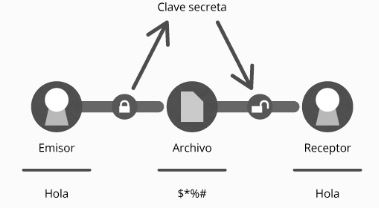
\includegraphics[width=10cm, height=5cm]{./images/Cripto_Simetrica.jpg}
	\caption{Diagrama de Criptografía Simétrica.}
	\label{fig:1-2-3}
\end{figure}
La sintaxis de un esquema de cifrado sim\'etrico, esta dada por la siguiente definición.
\begin{definition} 
Un esquema de cifrado sim\'etrico est\'a conformado por una tripleta de algoritmos 
$\sf \Pi=(Gen, Enc, Dec)$, definidos como se describe a continuación:
\begin{itemize}
\item  El algoritmo generador de claves $\sf Gen$ selecciona una llave  $K$ al azar del conjunto de llaves $\cal K$, esto se denotar\'a como $K \rand {\cal K}$.
Esta clave $K$  ser\'a usada por los algoritmos  $\sf Enc$ y $\sf Dec$, esta clave la compartir\'an  emisor y receptor. 
\item El algoritmo de cifrado $\sf Enc$, toma como entrada un texto en claro  $M \in {\cal M}$ y una clave $K$ generada por  $\sf Gen$  y regresa un texto cifrado $C \in {\cal C}$.  Usualmente esto se denota como $C \leftarrow {\sf Enc}_K(M)$.
 \item El algoritmo de descifrado $\sf Dec$, toma como entrada un texto cifrado $C$ y una llave $K$ y regresa $M$. Esta operaci\'on se denota por  $M \leftarrow {\sf Dec}_K(C)$.
Para que cualquier algoritmo de cifrado sim\'etrico funcione correctamente, se debe garantizar que para
todas las llaves posibles en  $\cal K$ y todos los posibles mensajes $\cal M$, $$ {\sf Dec}_K({\sf Enc}_K(M)) = M.$$
\end{itemize}
\end{definition}

\section{Criptografía asimétrica. }
La criptografía asimétrica es por definición aquella que utiliza dos claves diferentes para cada usuario, una para cifrar que se le llama clave pública y otra para descifrar que es la clave privada. Los algoritmos asimétricos son diferentes a los simétricos en un sentido muy importante ~\cite{sime}. Cuando se genera una clave simétrica, simplemente se escoge un número aleatorio de la longitud apropiada. Al generar claves asimétricas el proceso es más complejo. ~\cite{sime}.

\bigskip Características de la Criptografía asimétrica: \begin{itemize}
	\item Se basa en operaciones matemáticas complejas.
	\item Se ejecuta de 100 a 1000 veces más lento que los algoritmos simétricos.
\end{itemize} ~\cite{sime} \\ \\ 

 Los beneficios de la criptografía asimétrica son la solución a los problemas de la criptografía simétrica, pues las claves públicas pueden ser distribuidas con toda tranquilidad, no valen de nada sin las claves privadas. El cifrado asimétrico se emplea muy frecuentemente para pasar con seguridad una clave privada, que posteriormente, será la que se utilice para cifrar y/o descifrar otra información. El cifrado asimétrico puede ser representado como aparece en la figura ~\ref{fig:1-2-4}.

\begin{figure}[H]
\centering
	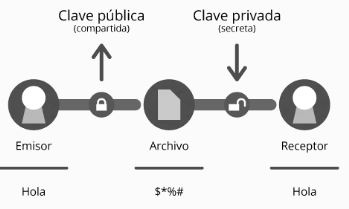
\includegraphics[width=10cm, height=5cm]{./images/Cripto_Asimetrica.jpg}
	\caption{Diagrama de Criptografía Asimétrica.}
	\label{fig:1-2-4}
\end{figure}

\section{Cifrado por bloques. }
Los algoritmos de cifrado por bloques toman bloques de tamaño fijo del texto en claro y producen un bloque de tamaño fijo de texto cifrado, generalmente del mismo tamaño que la entrada. El tamaño del bloque debe ser lo suficientemente grande como para evitar ataques de texto cifrado. La asignación de bloques de entrada a bloques de salida debe ser uno a uno para hacer el proceso reversible y parecer aleatoria.\\ 
Para la asignación de bloques los algoritmos de cifrado simétrico realizan sustituciones y permutaciones en el texto en claro hasta obtener el texto cifrado.\\ 
La sustitución es el reemplazo de un valor de entrada por otro de los posibles valores de salida, en general, si usamos un tamaño de bloque k, el bloque de entrada puede ser sustituido por cualquiera de los bloques posibles.
La permutación es un tipo especial de sustitución en el que los bits de un bloque de entrada son reordenados para producir el bloque cifrado, de este modo se preservan las estadísticas del bloque de entrada (el número de unos y ceros). \\ \\  Los algoritmos de cifrado por bloques iterativos funcionan aplicando en sucesivas rondas una transformación a un bloque de texto en claro. La misma función es aplicada a los datos usando una subclave obtenida de la clave secreta proporcionada por el usuario. El número de rondas en un algoritmo de cifrado por bloques iterativo depende del nivel de seguridad deseado.

La sustitución es el reemplazo de un bloque de $n$ bits por otro bloque de $n$ bits en un espacio de 
$2^{k}$~\cite{bloc}. Los cifradores por bloques mas usados son AES (Advanced Encryption Standard, por sus 
siglas en ingl\'es) y DES (Data Encryption Standard, por sus siglas en ingl\'es). ~\cite{bloques}\\ \\ 

Los cifradores por bloques pueden ser representados como se ve en la figura ~\ref{fig:1-2-5}.

\begin{figure}[H]
\centering
	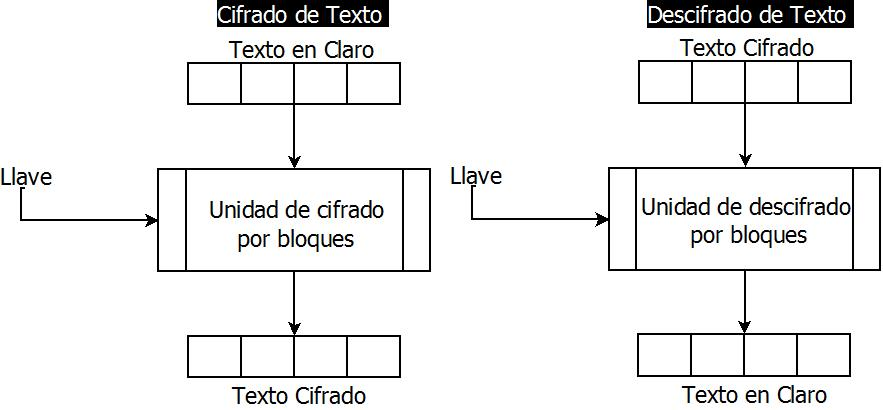
\includegraphics[width=10cm, height=5cm]{./images/CifradoBloques.jpeg}
	\caption{Diagrama de Cifradores por Bloques}
	\label{fig:1-2-5}
\end{figure}



%\section{Modos de operación. }
%Un modo de operación es una técnica para mejorar el efecto de un algoritmo criptográfico o adaptar el algoritmo para una aplicación, tal como aplicar un cifrador por bloques a una secuencia de bloques de datos o un flujo de datos. Los cuatro modos están destinados a cubrir virtualmente todas las aplicaciones posibles de cifrado para las cuales se podría usar un cifrador por bloques. A medida que han aparecido nuevas aplicaciones y requisitos, el NIST  (National Institute of Standards and Technology) ha ampliado la lista de modos recomendados a cinco en la Publicación Especial 800-38A. Estos modos están diseñados para usarse con cualquier cifrador por bloques bloques, incluyendo DES triple y AES.\\\\


%\textit{CBC}(Cipher-block chaining): La entrada al algoritmo de cifrado es el XOR de los siguientes 64 bits de texto plano y los 64 bits de cifrado anteriores.\\
%\begin{itemize}
%	\item La salida de uno de los bloques de cifrado se mete a otro bloque de cifrado junto con el siguiente bloque de mensaje.
%	\item Toma como entradas un vector de inicialización (IV) y un bloque de mensaje (m).
%	\item Durante el cifrado la salida del i - ésimo bloque depende del anterior i -1 bloques.
%	\item La salida de cada uno de los bloques depende de todo lo anterior y esto lo hace mas seguro que ECB.
%	\item  El descifrado de CBC es no secuencial.
%\end{itemize}

%\begin{figure}[h]
    %\centering
%    \begin{subfigure}[t]{0.5\textwidth}
    %    \centering
        %\includegraphics[height=3in]{./images/CBC.png}
%        \caption{Diagrama CBC Cifrado / Descfrado.}
    %    \label{fig:1-3-1}
%    \end{subfigure}
%\end{figure}
%\pagebreak

%\textit{CFB}(Cipher Feedback): La entrada se procesa j bits a la vez. El texto cifrado precedente se utiliza como entrada al algoritmo de cifrado para producir la salida pseudoaleatoria, que se le aplica XOR con el texto sin formato para producir la siguiente unidad de texto cifrado.\\
%\begin{itemize}
%	\item Los bloques de cifrado también están encadenados pero la salida es muy diferente a los demás.
%	\item Para cada bloque, el cifrado es producido haciendo XOR con el mensaje.
%	\item Una ventaja de implementación es que no es necesaria la operación de descifrar no es necesario.
%\end{itemize}

%\begin{figure}[h]
    %\centering
%    \begin{subfigure}[t]{0.5\textwidth}
    %    \centering
        %\includegraphics[height=3in]{./images/CFB.png}
     %   \caption{Diagrama CFB Cifrado}
        %\label{fig:1-3-1}
%    \end{subfigure}
%\end{figure}
%\pagebreak

%\textit{OFB}(Output feedback): Similar a CFB, excepto que la entrada al algoritmo de cifrado es la salida DES anterior.\\
%\begin{itemize}
%	\item En OFB la salida del bloque de cifrado es alimentada de nuevo en la siguiente bloque de cifrado.
%	\item El IV es cifrado varias veces para obtener una corriente de bytes aleatorios.
%	\item Estas corrientes de bytes aleatorios se les hace XOR con el texto en plano para generar el texto cifrado.
%\end{itemize}

%\begin{figure}[h]
%    \centering
    %\begin{subfigure}[t]{0.5\textwidth}
%        \centering
 %       \includegraphics[height=3in]{./images/OFB.png}
     %   \caption{Diagrama OFB Cifrado}
        %\label{fig:1-3-1}
%    \end{subfigure}
%\end{figure}
%\pagebreak

%\textit{CTR}(Counter): Cada bloque de texto sin formato se le aplica XOR con un contador cifrado. El contador se incrementa para cada bloque subsiguiente.\\
%\begin{itemize}
%	\item CTR toma un vector de inicialización (IV) y en cada iteración el valor de IV se incrementa en 1 y queda cifrado.
%	\item Para obtener el mensaje cifrado se hace una XOR con el IV y el bloque de mensaje.
%	\item En términos de eficiencia CTR es mejor que CBC, OFB o CFB, ya que en este modo se pueden hacer las operaciones en paralelo ya que no dependen de algo para poder ser cifradas.
%\end{itemize}

%\begin{figure}[h]
    %\centering
%    \begin{subfigure}[t]{0.5\textwidth}
    %    \centering
        %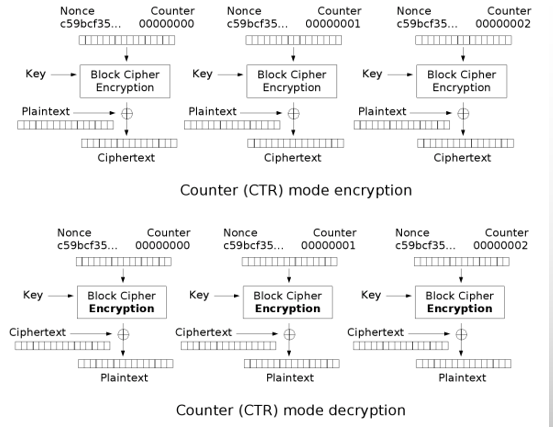
\includegraphics[height=3in]{./images/CTR.png}
%        \caption{Diagrama CTR Cifrado}
%        \label{fig:1-3-1}
    %\end{subfigure}
%\end{figure}

%\pagebreak

\section{RSA. }

El algoritmo de clave pública RSA fuecreado en 1978 por Rivest, Shamir y Adlman, y es el sistema criptográfico asimétrico más conocido y usado. Estos señores se basaron en el artículo de Diffie-Hellman sobre sistemas de llave pública, crearon su algoritmo y fundaron la empresa RSA Data Security Inc., que es actualmente una de las más prestigiosas en el entorno de la protección de datos.
El sistema RSA se basa en el hecho matemático de la dificultad de factorizar números muy grandes. Para factorizar un número el sistema más lógico consiste en empezar a dividir sucesivamente éste entre 2, entre 3, entre 4,..., y así sucesivamente, buscando que el resultado de la división sea exacto, es decir, de resto 0, con lo que ya tendremos un divisor del número.

Ahora bien, si el número considerado es un número primo (el que sólo es divisible por 1 y por él mismo), tendremos que para factorizarlo habría que empezar por 1, 2, 3,........... hasta llegar a él mismo, ya que por ser primo ninguno de los números anteriores es divisor suyo. Y si el número primo es lo suficientemente grande, el proceso de factorización es complicado y lleva mucho tiempo.

Basado en la exponenciación modular de exponente y módulo fijos, el sistema RSA crea sus claves de la siguiente forma:
\begin{itemize}

	\item Se buscan dos números primos lo suficientemente grandes: p y q (de entre 100 y 300 dígitos).
	\item Se obtienen los números n = p * q y Ø = (p-1) * (q-1).
	\item Se busca un número e tal que no tenga múltiplos comunes con Ø.
	\item Se calcula d = e-1 mod Ø, con mod = resto de la división de números enteros. Y ya con estos números obtenidos, n es la clave pública y d es la clave privada. Los números p, q y Ø se destruyen. También se hace público el número e, necesario para alimentar el algoritmo.
\end{itemize} 

El cálculo de estas claves se realiza en secreto en la máquina en la que se va a guardar la clave privada, y una vez generada ésta conviene protegerla mediante un algoritmo criptográfico simétrico.

En cuanto a las longitudes de claves, el sistema RSA permite longitudes variables, siendo aconsejable actualmente el uso de claves de no menos de 1024 bits (se han roto claves de hasta 512 bits, aunque se necesitaron más de 5 meses y casi 300 ordenadores trabajando juntos para hacerlo).

RSA basa su seguridad es ser una función computacionalmente segura, ya que si bien realizar la exponenciación modular es fácil, su operación inversa, la extracción de raices de módulo Ø no es factible a menos que se conozca la factorización de e, clave privada del sistema.

RSA es el más conocido y usado de los sistemas de clave pública, y también el más rápido de ellos. Presenta todas las ventajas de los sistemas asimétricos, incluyendo la firma digital, aunque resulta más útil a la hora de implementar la confidencialidad el uso de sistemas simétricos, por ser más rápidos. Se suele usar también en los sistemas mixtos para encriptar y enviar la clave simétrica que se usará posteriormente en la comunicación cifrada. ~\cite{rsa}

\section{Firmas a ciegas. }

Las firmas a ciegas son un tipo especial de firmas digitales en las que se firma algo que no se conoce. Para hacer firmas a ciegas se utilizan factores de opacidad, para ocultar el mensaje original que se requiere que est´e firmado, y as´ı la autoridad no pueda conocer lo que est´a firmando.
Por lo tanto, el prop´osito de una firma a ciegas es evitar que el firmante B conozca el mensaje que firma; y as´ı posteriormente, sea incapaz de asociar el mensaje que firm´o con el remitente A. Entonces, las firmas a ciegas tienen aplicaci´on en varias situaciones. A continuaci´on se mencionan dos de ellas:
\begin{itemize}
	\item Cuando se utiliza dinero electr´onico. En este caso, m representa un valor monetario que A (el cliente) tiene derecho a gastar. Y as´ı, cuando m y s(m) se presentan a B (el banco) para efectuar el pago, B es incapaz de identificar al cliente que originalmente le dio ese dinero electr´onico a firmar, pues le fue enviado de manera oculta. Lo anterior permite que la identidad de A 	permanezca an´onima, y sus movimientos financieros no puedan ser monitoreados.
	\item En las elecciones electr´onicas tambi´en pueden utilizarse las firmas a ciegas, ya que se requiere que B (una autoridad electoral) no conozca la identidad de A (el votante) debido a que el voto debe efectuarse de manera an´onima. Sin embargo, es necesario que A demuestre que su voto m es v´alido. Lo cual se logra cuando A presenta ante B la firma s(m). Y se sabe de antemano que B no puede asociar s(m) a A, debido a que el votante previamente le env´ıo a B su voto m pero de forma oculta para que se lo firmara. ~\cite{ciegas}
\end{itemize} 

\section{Funciones Hash. }
A continuaci\'on se describir\'an las caracter\'isticas de las {\it funciones hash}, tambi\'en conocidas como {\it funciones de resumen}. Las funciones hash basan su definici\'on en funciones de un solo sentido  ({\it one-way functions}, en ingl\'es). Una funci\'on de un s\'olo sentido es aquella que para un valor $x$, es  muy f\'acil calcular $f(x)$, pero es muy dif\'icil hallar $f^{-1}(x)$. Es complicado en general, hallar funciones de \'este tipo y probar que lo son.
\begin{definition}
Una funci\'on hash, es una funci\'on de un s\'olo sentido cuya entrada $m$  es un mensaje de longitud arbitraria y la salida es una cadena binaria de longitud fija. Al resumen o hash de un mensaje $m$, se le denotar\'a como $h(m)$. Una funci\'on hash debe
tener las siguientes propiedades:
\begin{itemize}
	\item Para cualquier mensaje $m$, debe ser posible calcular $h(m)$ eficientemente. 
	\item Dado $h(m)$, debe ser computacionalmente dif\'icil, hallar un mensaje $m'$, tal que $h(m)=h(m')$.
	\item Debe ser computacionalmente dif\'icil, hallar dos mensajes $m$ y $m'$ tales que $h(m)=h(m')$.
\end{itemize}
\end{definition}
 
Entre las funciones hash que se usan para criptograf\'ia est\'an: MD2, MD4, MD5, donde MD significa {\it Message Digest}, y el algoritmo est\'andar al momento de escribir \'estas notas es el {\it Secure Hash Algorithm} por sus siglas en ingl\'es SHA.
  La MD5 fue dise\~nada por Ron Rivest, toma como entrada un mensaje de longitud arbitraria y proporciona como salida una cadena binaria de 128 bits.
El mensaje de entrada se procesa por bloques de 512 bits.  La SHA 256 fue dise\~nada por en NIST (National Institute of Standards and Technology) y se estableci\'o como est\'andar en 1993. Recibe como entrada un mensaje con longitud menor a $2^{64}$ bits y
como salida se obtiene una cadena binaria de 160 bits. Al igual que el MD5, se procesa en bloques de 512 bits ~\cite{modes}.


\section{Cómputo Nube. }
El cómputo nube definido así por el NIST, es un modelo para permitir un acceso a la red ubicuo, es decir, que se encuentra presente en todas partes al mismo tiempo y conveniente a un conjunto de recursos informáticos configurables (por ejemplo, redes, servidores, almacenamiento, aplicaciones y servicios) que se puede aprovisionar y liberar rápidamente con un esfuerzo mínimo de gestión o una interacción entre el proveedor de servicios.
Este modelo de cómputo nube se compone de 5 características esenciales, 3 modelos de servicio y 4  modelos de despliegue. \\ \\  

\textbf{Características: }
\begin{itemize}
	\item \textbf {Auto-servicio bajo demanda. } \\  Un consumidor puede proporcionar unilateralmente capacidades del tiempo del servidor y el almacenamiento en red, según se necesite automáticamente sin interacción con cada proveedor de servicios.
 	\item \textbf {Amplio acceso a la red. } \\   Las capacidades están disponibles a través de la red y se accede a través de mecanismos que promueven el uso por plataformas de clienteheterogéneas finas o gruesas (por ejemplo, teléfonos móviles, tablets, computadoras portátiles y estaciones de trabajo)
	\item \textbf {Agrupación de recursos. } \\ Los recursos informáticos del proveedor se agrupan para servir a múltiples consumidores utilizando un modelo de múlti- usuario, con diferentes recursos físicos y virtuales asignados dinámicamente y reasignados de acuerdo con la demanda del consumidor. Hay una sensación de independencia de ubicación en que el cliente generalmente no tiene control o conocimiento sobre la ubicación exacta de los recursos proporcionados, pero puede especificar la ubicación en un nivel superior de abstracción (por ejemplo, país, estado o centro de datos). Ejemplos de recursos incluyen almacenamiento, procesamiento, memoria y ancho de banda de la red.
	\item \textbf{Elasticidad rápida. } \\ Las capacidades pueden ser suministradas elásticamente y liberadas, en algunos casos de forma automática, para escalar rápidamente hacia fuera y hacia adentro proporcional a la demanda. Para el consumidor, las capacidades disponibles para la provisión a menudo parecen ser ilimitadas y pueden ser apropiadas en cualquier cantidad en cualquier momento.
	\item \textbf{Servicio medido. } \\ Los sistemas de cómputo nube controlan y optimizan automáticamente el uso de recursos aprovechando una capacidad de medición en algún nivel de abstracción apropiado al tipo de servicio (por ejemplo, almacenamiento, procesamiento, ancho de banda y cuentas de usuario activas). El uso de recursos puede ser monitoreado, controlado y reportado, proporcionando transparencia tanto para el proveedor como para el consumidor del servicio utilizado.
\end{itemize}    

 \textbf{Modelos de servicio. }

\begin{itemize}
	\item \textbf {Software como Servicio (SaaS). } \\ La capacidad proporcionada al consumidor es utilizar las aplicaciones del proveedor que se ejecutan en una infraestructura en la nube. Las aplicaciones son accesibles desde varios dispositivos cliente a través de una interfaz de cliente ligero, como un navegador web (por ejemplo, correo electrónico basado en web) o una interfaz de programa. El consumidor no gestiona ni controla la infraestructura oculta de la nube, incluyendo la red, los servidores, los sistemas operativos, el almacenamiento o incluso las capacidades de las aplicaciones individuales, con la posible excepción de las limitadas configuraciones específicas de la configuración de la aplicación.
	\item \textbf {Plataforma como Servicio (PaaS). } \\ La capacidad proporcionada al consumidor es desplegar en la infraestructura de la nube aplicaciones creadas por el consumidor, utilizando lenguajes de programación, bibliotecas, servicios y herramientas soportadas por el proveedor. El consumidor no gestiona ni controla la infraestructura oculta de la nube, incluyendo la red, los servidores , sistemas operativos o de almacenamiento, pero tiene control sobre las aplicaciones desplegadas y, posiblemente, configuración de configuración para el entorno de alojamiento de aplicaciones.
	\item \textbf {Infraestructura como Servicio (IaaS). } \\  La capacidad proporcionada al consumidor es proveer procesamiento, almacenamiento, redes y otros recursos de computación fundamentales donde el consumidor es capaz de desplegar y ejecutar software arbitrario, que puede incluir sistemas operativos y aplicaciones. El consumidor no gestiona ni controla la infraestructura subyacente de la nube, sino que tiene control sobre los sistemas operativos, el almacenamiento y las aplicaciones implementadas; Y posiblemente un control limitado de componentes de red selectos (por ejemplo, firewalls de host). 
\end{itemize}  

 \textbf{Modelos de despliegue. }
\begin{itemize}
	\item \textbf {Nube privada. } \\ La infraestructura de la nube está preparada para el uso exclusivo de una sola organización que comprende varios consumidores (por ejemplo, unidades de negocio). Puede ser propiedad, administrado y operado por el órgano.
	\item \textbf{Nube de la comunidad. } \\ La infraestructura de la nube está preparada para uso exclusivo por una comunidad específica de consumidores de organizaciones que tienen preocupaciones compartidas (por ejemplo, misión, requisitos de seguridad, política y consideraciones de cumplimiento). Puede ser propiedad, administrado y operado por una o más de las organizaciones de la comunidad, un tercero, o una combinación de ellos, y puede existir dentro o fuera de las instalaciones.
	\item \textbf{Nube pública. } \\ La infraestructura de la nube está preparada para el uso abierto por el público en general. Puede ser propiedad, administrado y operado por una organización comercial, académica u gubernamental, o alguna combinación de ellos. Existe en las instalaciones del proveedor de la nube.
	\item \textbf{Nube híbrida. } \\  La infraestructura de la nube es una composición de dos o más infraestructuras de nube distintas (privadas, comunitarias o públicas) que siguen siendo entidades únicas, pero están unidas por una tecnología estandarizada o propietaria que permite la portabilidad de datos y aplicaciones (por ejemplo, burbujas de nube para equilibrar la carga entre Nubes).
\end{itemize}   


 \textbf{Problemas en Cómputo Nube. }

\begin{itemize}
	%\item \textbf {Abuso y mal uso del Cómputo Nube. } \\ Esta amenaza afecta principalmente a los modelos de servicio IaaS y PaaS y se relaciona con un registro de acceso a estas infraestructuras/plataformas poco restrictivo. Es decir, cualquiera con una tarjeta de crédito válida puede acceder al servicio, con la consecuente proliferación de spammers, creadores de código malicioso y otros criminales que utilizan la nube como centro de operaciones. 
	\item \textbf {Interfaces y API poco seguros. } \\ Generalmente los proveedores de servicios en la nube ofrecen una serie de interfaces y API (del inglés, Application Programming Interface) para controlar e interactuar con los recursos. De este modo, toda la organización, el control, la provisión y la monitorización de los servicios cloud se realiza a través de estos API o interfaces. 
Dado que todo (autenticación, acceso, cifrado de datos, etc.) se realiza a través de estas herramientas, se hace necesario que los interfaces estén diseñados de forma segura, evitando así los problemas de seguridad, tanto los que son intencionados como los que se producen de forma accidental. 
	%\item \textbf {Amenaza Interna. } \\ Como en todos los sistemas de información, la amenaza que suponen los propios usuarios es una de las más importantes, dado que tienen acceso de forma natural a los datos y aplicaciones de la empresa. En un entorno cloud esto no es en absoluto diferente ya que se pueden desencadenar igualmente incidentes de seguridad provocados por empleados descontentos y accidentes por error o desconocimiento. 
%Además, en muchos casos, es el propio proveedor del servicio el que gestiona las altas y bajas de los usuarios, produciéndose brechas de seguridad cuando el consumidor del servicio no informa al proveedor de las bajas de personal en la empresa. 
%Como es lógico, estos incidentes repercuten de forma importante en la imagen de la empresa y en los activos que son gestionados. 
%Los proveedores de servicio deberán proveer a los consumidores del servicio de medios y métodos para el control de las amenazas internas.
	%\item \textbf {Problemas derivados de la tecnología compartida. } \\  Esta amenaza afecta a los modelos IaaS, ya que en un modelo de Infraestructura como Servicio los componentes físicos (CPU, GPU, etc.) no fueron diseñados específicamente para una arquitectura de aplicaciones compartidas. Se han dado casos en los que los hipervisores de virtualización podían acceder a los recursos físicos del anfitrión provocando, de esta forma, incidentes de seguridad. 
%Para evitar este tipo de incidentes se recomienda implementar una defensa en profundidad con especial atención a los recursos de computación, almacenamiento y red. Además, se ha de generar una buena estrategia de seguridad que gestione correctamente los recursos para que las actividades de un usuario no puedan interferir en las del resto. 
	\item \textbf {Pérdida o fuga de información. } \\ Existen muchas formas en las que los datos se pueden ver comprometidos. Por ejemplo, el borrado o modificación de datos sin tener una copia de seguridad de los originales, supone una pérdida de datos. 
En la nube, aumenta el riesgo de que los datos se vean comprometidos ya que el número de interacciones entre ellos se multiplica debido a la propia arquitectura de la misma. Esto deriva en pérdida de imagen de la compañía, daños económicos y, si se trata de fugas, problemas legales, infracciones de normas, etc.
	\item \textbf {Secuestro de sesión o servicio. } \\  En un entorno en la nube, si un atacante obtiene las credenciales de un usuario del entorno puede acceder a actividades y transacciones, manipular datos, devolver información falsificada o redirigir a los clientes a sitios maliciosos.
	%\item \textbf {Riesgos por desconocimiento. } \\ Uno de los pilares de las infraestructuras cloud es reducir la cantidad de software y hardware que tienen que adquirir y mantener las compañías, para así poder centrarse en el negocio. Esto, si bien repercute en ahorros de costes tanto económicos como operacionales, no puede ser motivo para el deterioro de la seguridad por falta de conocimiento de esta infraestructura. 
%Para asistir en la toma de decisiones sobre las medidas de seguridad que se han de implantar en un entorno cloud es conveniente conocer, al menos en parte, la información técnica de la plataforma. Datos como con quién se comparte la infraestructura o los intentos de acceso no autorizados pueden resultar muy importantes a la hora de decidir la estrategia de seguridad. 
%La carencia de información de este tipo puede derivar en brechas de seguridad desconocidas por el afectado. 
\end{itemize} 


%Las funciones hash son usadas para construir una pequeña huella digital de la informaci\'on, si la informaci\'on es alterada tambi\'en la huella digital es alterada. Esta caracter\'istica hace que las funciones hash sean ampliamente usadas para verificar la integridad de datos.\\
%De manera formal, un funci\'on Hash es una Cuadrupla$(X,Y,K,H)$ donde:
%\begin{enumerate}
% \item $X$ es un conjunto de posibles mensajes.
% \item $Y$ es un conjunto finito de posibles resúmenes de mensajes o etiquetas de autenticación.
% \item $K$, el espacio de claves, es un conjunto finito de posibles claves.
% \item Para cada $k\quad \epsilon\quad K$, existe una función hash $h_k\quad \epsilon\quad H$. Parac ada $h_k: X \longrightarrow Y$.
% \cite{stinson}
%\end{enumerate}




\chapter{Adversarios Clasificadores}



Los adversarios clasificadores son programas de c\'omputo que se dedican a observar  mensajes que se intercambian  entre  los  usuarios  de  correo  electrónico,  con  el  fin  de  clasificarlos  e 
identificar  a  todos  los  usuarios  que  cumplan  con  cierto  criterio.  Esta  clasificación  se hace de manera masiva a trav\'es de  una búsqueda de palabras clave dentro de 
los  mensajes de  los usuarios. Por ejemplo, el  clasificador puede estar interesado en  los mensajes  que  contienen  la  palabra  clave  "Bomba",  así  que 
todos  los  mensajes  que contengan esta palabra serán etiquetados en una clasificación en específico, este proceso se lleva a cabo por medio de técnicas de 
“Reconocimiento de patrones” y “Aprendizaje Máquina” para encontrar y clasificar los mensajes 
que intercepta~\cite{clas,Attacks}.
\\
La  clasificación  de  estos  mensajes  tiene  diversos  usos, ya  que  pueden  ser  clasificados con  fines demográficos, con  fines comerciales o con  fines gubernamentales. Todo esto 
con  el  propósito  de  generar  las  estadísticas  de  comportamientos  e  intereses  de  los usuarios de correo electrónico. \\




En este trabajo terminal, se considera que un adversario clasificador solo es capaz de realizar ataques de solo texto cifrado (ciphertext only attack, en ingl\'es). Como se mencion\'o en el cap\'itulo anterior, en este ataque  el adversario solo  cuenta  con  los  textos  cifrados  que  va  recopilando  de  un  canal  o  base  de 
datos. Posteriormente, el adversario utiliza  estos  textos  cifrados  para  hacer  un  análisis  criptográfico  de  cómo  se comporta la técnica de cifrado  y tratar de hallar el texto en claro a partir de los textos cifrados que va recopilando. 
\\
Este  tipo  de  ataques  es  muy  común  en  el  internet  aunque  con  muy  baja  efectividad cuando   se   implementa   en   comunicaciones   altamente   protegidas,   y   cuando   se 
implementa en canales de comunicación desprotegidos  la  información obtenida  llega  a ser  muy  pobre.  En  los  últimos  años  se  han  dado  cuenta  que  si   este  tipo  de 
adversarios   atacan las  comunicaciones  sin  cifrado se  obtienen  características  valiosas  sobre  los usuarios  que  utilizan  este  tipo  de  canales  de  comunicación,  este  tipo  de  ataques  son 
ejecutados por  adversarios clasificadores.\\


\subsection{Esquema Golle - Farahat}
La  única  referencia  que se tiene  sobre  un  esquema  criptográfico  contra  adversarios clasificadores es el que propusieron Golle y Farahat~\cite{Attacks}. En este art\'iculo se habla por primera vez de las caracter\'isticas de este tipo de adversarios  y se considera la posibilidad de utilizar un esquema de cifrado con un nivel de seguridad menor.
%en el artículo 
%“Defending Email Communication Against Profiling” de Philippe Golle  y  Ayman  Farahat, ambos  miembros del 
%“Palo Alto Research Center”.\cite{Attacks}\\
%En su artículo se aborda el ataque de adversarios clasificadores sobre los mensajes de correo electrónico, en el cual se proponen un protocolo para la comunicación por correo electrónico. 
Golle y Farahat proponen un protocolo que hace uso de una función  de cifrado, el cual sustituye cada una de las palabras del mensaje por otra de la misma extensión y frecuencia gramatical, esta función esta pensada para textos en idioma ingl\'es. 
%Esta función tiene como parámetro una clave $K$.  
Para cifrar se utiliza una clave que se genera  usando los datos de cabecera que acompañan al mensaje los cuales pueden ser dirección  del remitente, la dirección del destinatario, la hora a la que se envía el correo electrónico y potencialmente otros campos. Estos datos se introducen en una función hash lenta y el resultado de esta función es la clave $K$. Estas funciones hash  tiene con una complejidad de c\'alculo moderadamente mas alta que las 
funciones hash est\'andar.  \\
Este  protocolo resulta inseguro para la criptografía moderna pero es efectivo contra el ataque de clasificadores. Por otro lado este protocolo resuelve dos problemas, le  permite  a los usuarios  calcular  la  clave de cifrado y descifrado  fácilmente  ya  que  los datos del mensaje con que se calcula son  públicos, resolviendo así el intercambio de claves. Al usar un cifrado de tipo semántico se permite que el texto se vea como un texto en inglés pero indistinguible para los clasificadores y por lo tanto este clasifica incorrectamente el mensaje cifrado.\\

\section{CAPTCHA}
 Es un programa informático diseñado para diferenciar un ser humano de una computadora, CAPTCHA son las siglas de prueba de Turing completamente automática y pública para diferenciar computadoras de humanos ({\it Completely Automated Public Turing test to tell Computers and Humans Apart} por sus siglas en ingl\'es).  Un CAPTCHA es una prueba que es fácil de pasar por un usuario humano pero difícil de pasar por una máquina. Uno de los CAPTCHAs más com\'unes son imágenes distorsionadas de cadenas cortas de caracteres. Para un humano es generalmente muy fácil recuperar la cadena original de la imagen distorsionada, pero es difícil para  los algoritmos de reconocimiento de caracteres recuperar la cadena original de la imagen distorsionada.\\
Un CAPTCHA en un algoritmo aleatorio $G$, que recibe como parámetro una cadena de caracteres STR y produce como resultado un CAPTCHA $G(x)$\\

\begin{figure}[H]
\centering
	
\includegraphics[width=5cm, height=3cm]{./images/cptc.jpeg}
	\caption{CAPTCHA}
	\label{fig:3-6}
\end{figure}
 
%La criptografía moderna se basa en dos corrientes metodológicas que son la criptografía simétrica  y  la criptografía asimétrica. Estas dos técnicas tienen como propósito ocultar 
%el  contenido  de  un  mensaje  con  el  fin  de  que  solo  sea  leído  por  aquellos  que  estén autorizados, a esto se le llama cifrado. 




\section{Esquema de Secreto Compartido de Shamir}
El esquema de secreto compartido fue propuesto por Adi Shamir en 1997\cite{shamir}. 
El objetivo de este método es dividir un secreto $K$ en $w$ partes,que son dadas a $w$ participantes. Para recuperar el secreto es necesario tener al menos $u$
elementos de las $w$ partes siendo $u \leq w$. Y no es posible recuperar el secreto si se tienen menos que $u$ partes.

Para construir el esquema del secreto compartido primero es necesario seleccionar un número primo $p \geq w+1$ el cual define al conjunto $\mathbb{Z}_p$.
\\
\\
El procedimiento para dividir un secreto $K$ en $w$ partes es el siguiente:

\begin{enumerate}
 \item Se seleccionan $w$ elementos distintos de cero del conjunto $\mathbb{Z}_p$ denotados como $x_i$ donde $1 \leq i \leq w$.
 \item Se seleccionan $u-1$ elementos aleatorios de $\mathbb{Z}_p$ denotados como $a_1,...,a_{u-1}$.
 \item Se construye el polinomio $y_x$ de la siguiente forma. Sea \begin{equation}
            y(x)=K+\sum_{j=1}^{u-1} a_j x^j \bmod \quad p
           \end{equation}
           Por medio de este polinomio se calculan los elementos $y_i$.
 \item La salida es el conjunto $S=\{(x_1,y_1),...,(x_w,y_w)\}$.
\end{enumerate}

Para recuperar el secreto solo tenemos que resolver un sistema de ecuaciones  que es definido por el polinomio característico $a(x)=a_0+a_1x+...+a_{u-1}x^{u-1}$.
\\
\\
Posteriormente se seleccionan $u$ pares de elementos $(x_w,y_w)$ con los que obtendremos nuestro sistema de ecuaciones a resolver. El elemento que nos interesa obtener del sistema de ecuaciones es $a_0$ ya que este es el valor de nuestro secreto $K$.
\begin{example}
Si se considera el conjunto  $\mathbb{Z}_{11}$ y se desea compartir el secreto $K=8$, entre 5 participantes,
de tal manera que solo cuando se re\'unan cualesquiera 2 de ellos sea posible recuperar $K$, es decir
 $w=5$ y $u=2$.

Se seleccionan los $u-1$ elementos del conjunto $\mathbb{Z}_{11}$, puesto que $u=2$ en este caso solo 
hay que escoger un elemento: $a_1=5$.

A continuaci\'on se seleccionan $w$ elementos de $\mathbb{Z}_{11}$, por ejemplo 
 $x_1=2, x_2=7, x_3=9, x_4=10, x_5=3$.

Posteriormente, se calcula el conjunto de elementos $y_i$ por medio de la ecuaci\'on 
\begin{equation} \nonumber
 y_i=k+\sum_{j=1}^{u-1} a_j x_i^j \bmod \quad p
\end{equation}

En el caso del ejemplo, la ecuaci\'on anterior queda como sigue:

\begin{equation} \nonumber
 y_i=K+a_1x_i \bmod \quad p
\end{equation}
Y se obtienen los siguientes valores:
$$\begin{array}{lcl}
y_1&=&8+5(2) \bmod 11=7, \\
y_2&=&8+5(7) \bmod 11=10,\\
y_3&=&8+5(9) \bmod 11=9, \\ 
y_4&=&8+5(10) \bmod11=3, \\
y_5&=&8+5(3) \bmod 11=1. 
\end{array}$$

Finalmente, se tienen los pares $S=\{ (2,7), (7,10), (9,9), (10,3),(3,1)\}$
%$A_1(2,7)$\hspace{1cm}$A_2(7,10)$\hspace{1cm}$A_3(9,9)$\hspace{1cm}$A_4(10,3)$\hspace{1cm}$A_5(3,1)$\\


Para recuperar la llave $K$ es necesario seleccionar $u=2$ pares del conjunto $S$, por ejemplo
$A_2(7,10)$, $A_4(10,3)$. Con estos pares se puede crear el siguiente  sistema de ecuaciones:
$$\begin{array}{lcl}
 a_0+a_1x_2&=&y_2 \\
 a_0+a_1x_4&=&y_4 
 \end{array}$$
 Es importante notar, que en tal sistema de ecuaciones, las inc\'ognitas son $a_0$ y $a_1$, las cuales
 son desconocidas para los $w$ participantes.  Para el esquema de secreto compartido de
 Shamir, es de particular inter\'es $a_0$, ya que  $a_0=K$.
Al sustituir los pares $A_2$ y $A_4$ en el sistema de ecuaciones anterior, se tiene:
\begin{align}
a_0+7a_1&=10 \label{eq-3}\\
a_0+10a_1&=3 \label{eq-4}
\end{align}
Para resolver este sistema se puede utilizar cualquiera de los métodos com\'unes que se usan en álgebra, solo que respetando el conjunto $\mathbb{Z}_p$, en este caso se resolverá por el método suma y resta.\\
%\begin{equation*}
% a_0+7a_1=10
%\end{equation*}
%\begin{equation}
% a_0+10a_1=3
%\end{equation}
Multiplicamos la ecuación~(\ref{eq-3}) por $-1$ y obtenemos:
\begin{equation}
 -a_0-7a_1=-10 \label{eq-5}
\end{equation}
%\begin{equation}
% a_0+10a_1=3
%\end{equation}
sumamos la ecuación~(\ref{eq-4}) con (\ref{eq-5})  d\'andonos como resultado:
\begin{equation} \nonumber
 3a_1=4
\end{equation}
de donde es posible despejar$a_1$
\begin{equation}
 a_1=\frac{4}{3} \label{eq-8}
\end{equation}
Puesto que 4 es el inverso multiplicativo de 3,  la ecuación~(\ref{eq-8}) queda de la siguiente forma
\begin{equation} \nonumber
 a_1=(4)(4)=16 \bmod 11 =5
\end{equation}
Sustituimos $a_1$ en la ecuación~(\ref{eq-4}) 
\begin{equation} \nonumber
 a_0+10(5)=3
\end{equation}
Simplificamos y despejamos $a_0$
\begin{align*}
 a_0+(50 \bmod 11)=3 \\
  a_0=-3 \bmod11=8
\end{align*}
Como $a_0=8$ podemos ver que se recuper\'o a $K$ exitosamente ya que  $a_0=K$.
\end{example}


\section{Esquema Díaz - Chakraborty}
Otro esquema para combatir a los adversarios clasificadores fue propuesto en 2012 por D\'iaz y 
Chakraborty~\cite{clas}.  El esquema D\'iaz-Chakraborty utiliza CAPTCHAs y un algoritmo de clave secreta,
para  proteger el correo electr\'onico. 
 Para obtener la clave se genera una cadena al azar, a la se le aplica una funci\'on hash, con esta clave se cifra el
 mensaje.  Tanto el mensaje cifrado como el CAPTCHA se env\'ian al receptor. El receptor debe
resolver el CAPTCHA, para obtener la cadena, aplicarle la funci\'on hash y as\'i obtener la clave de cifrado. Puesto que un adversario clasificador es un programa de c\'omputo, no podr\'a resolver un CAPTCHA y por tanto no podr\'a obtener la clave de cifrado.  Este esquema se muestra en la Figura~\ref{fig:protocol}.

\begin{figure}[h]
\centering
%\subfigure{
\begin{tabular}{|l|}
\hline
\begin{minipage}{220pt}
\begin{tabbing}
\ \ \ \ \ \=\ \ \ \ \=\ \ \ \ \=\ \ \ \ \=\ \ \ \ \=\ \ \ \ \=\ \ \
\ \kill \\
\ \ \ \ {\bf Protocol} ${\mathbb P}(x)$\\
\> 1. \> $k\rand {\sf STR}$; \\
\> 2. \> $k^{\prime} \leftarrow G(k)$; \\
\> 3. \> $K \leftarrow H(k)$; \\
\> 4. \> $c\leftarrow E_K(x)$;\\
\> 5. \> {\bf return} $(c, k^{\prime})$
\end{tabbing}
\end{minipage}\\
\hline
\end{tabular}
\caption{\label{fig:protocol} Protocol D\'iaz-Chakraborty.}
\end{figure}

 
%\begin{enumerate}
% \item \textbf{Esquema P}: Se genera una cadena de caracteres aleatoriamente llamada STR la cual es introducida a una funcion Hash para generar la clave $K$, con esta clave se cifra el mensaje original $M$. La cadena STR es convertida en un CAPTCHA y se envía junto con el texto cifrado al destinatario.\\\\
% \textbf{Esquema} P(x)
% \begin{enumerate}
%  \item $k\longleftarrow^\$ STR;$
%  \item $k'\longleftarrow G(k);$
%  \item $K\longleftarrow H(k);$
%  \item $c\longleftarrow E_k(x);$
%  \item $return(c,k')$
% \end{enumerate}
 Contemplando que es muy común que el usuario no consiga resolver el CAPTCHA D\'iaz y Chakraborty propusieron una variante del esquema anterior, el cual se describe a continuaci\'on. 
 Se genera una cadena de caracteres aleatoriamente llamada STR la cual se codifica a un valor entero. El valor entero es dividido en 5 pares $(x,k')$ por medio del algoritmo de Secreto Compartido, cada uno de los elementos $k'$ de los pares generados es decodificado a su correspondiente valor en cadena de caracteres para posteriormente ser convertidos en CAPTCHAS. Para finalizar la cadena STR se introduce en una función Hash para generar la llave $K$. Con esta llave se cifra el mensaje de correo y se envía junto con los pares de $(x,CAPTCHA)$.
Este esquema se puede observar en la Figura~\ref{fig:P-with-sharing}.
\begin{figure}[h]
\begin{center}
\begin{tabular}{|l|}
\hline
\begin{minipage}{220pt}
\begin{tabbing}
\ \ \ \ \ \=\ \ \ \ \=\ \ \ \ \=\ \ \ \ \=\ \ \ \ \=\ \ \ \ \=\ \ \
\ \kill \\
\ \ \ \ {\bf Protocol} ${\mathbb P}^{\prime}(x)$\\
\> 1. \> $k\rand {\sf STR}$; \\
\> 2. \> $k^\prime \leftarrow {\sf ENCD}(k,0);$\\
\> 3. \> $\{ (x_1, k_1^\prime), \ldots, (x_w, k_w^\prime)\} \leftarrow {\sf SHARE}^p_{u,w}(k^\prime)
$; \\
\> 4. \> {\bf for} $i=1$ {\bf to } $w$; \\
\> 5. \>\> $(k_i, \lambda_i) \leftarrow {\sf ENCD}^{-1}(k_i^\prime)$; \\
\> 6. \>\> $c_i \leftarrow G(k_i)$; \\
\> 7. \>{\bf end for} \\
\> 8. \> $K \leftarrow H(k)$; \\
\> 9. \> $C\leftarrow E_K(x)$; \\
\> 10. \> \hspace*{2mm}{\bf return} $[C,\{ (x_1, c_1, \lambda_1), \ldots, (x_w,
c_w, \lambda_w)\}]$
\end{tabbing}
\end{minipage}\\
\hline
\end{tabular}
\end{center}
\caption{\label{fig:P-with-sharing} Variante del  protocolo D\'iaz-Chakraborty}
\end{figure} 


% \begin{enumerate}
%  \item $k\longleftarrow^\$STR;$
%  \item $k'\longleftarrow ENCD(k);$
%  \item $\{(x_1,k'_1),...,(x_w,k'_w)\}\longleftarrow SHARE^p_{u,w}(k');$
%  \item $for\quad i=1\quad to \quad w;$
%  \item $\quad (k_i)\longleftarrow ENCD^{-1}(k'_1);$
%  \item $\quad c_i\longleftarrow G(k_i);$
%  \item $end for$
%  \item $K\longleftarrow H(k);$
%  \item $C\longleftarrow E_k(x);$
%  \item $return [C,\{(x_1,c_1),...,(x_w,c_w)\}]$
% \end{enumerate}


Este nuevo esquema se cre\'o pensando en que el usuario pueda tener más oportunidades de recuperar el mensaje cifrado y esto sucede gracias a el algoritmo de Secreto Compartido, ya que no este podemos tener la misma llave repartida en $n$ CAPTCHAS. A continuaci\'on se describe las funciones {\sf ENCD} y ${\sf ENCD}^{-1}$, cuyo
prop\'osito es convertir una cadena de caracteres a enteros y viceversa. 

\subsection{Codificaci\'on de caracteres a enteros}
Se tiene un conjunto de caracteres $AL$ compuesto por $AL=\{A,B,...,Z\}\cup\{a,b,...,z\}\cup\{0,1,...,9\}\cup\{+,/\}$ con una cardinalidad $|AL|=64$.

Para obtener una representación binaria de 64 elementos son necesarios 6 bits por lo que para todos los elementos $\sigma\epsilon AL$ existe una cadena binaria. Una vez establecido esto el procedimiento para realizar la conversión es el siguiente:
\begin{enumerate}
 \item Tomamos una cadena de caracteres y la separamos caracter por caracter y los intercambiamos por su correspondiente número entero en $AL$ $\alpha _0||\alpha _1||...||\alpha _m$
 \item Posteriormente cada uno de los enteros lo convertimos en un binario de 6 bits y se concatenan uno detrás del otro $\Psi\longleftarrow bin_6(\alpha _0)||bin_6(\alpha _1)||...||bin_6(\alpha _m$
 \item La cadena binaria $\Psi$ la convertimos a entero $v\longleftarrow toInt(\Psi)$
\end{enumerate}
\textbf{Ejemplo}:\\
Tenemos la cadena $STR=`ABC`$ de la cual cambiaremos cada caracter por su correspondiente valor entero en $AL$ quedando de la siguiente manera $\alpha =\{0,1,2\}$
\\ 
\\
Ahora cada  uno de los elementos de $\alpha$ lo convertiremos a su correspondiente representacion binaria, $bin_6(0)=000000, bin_6(1)=000001, bin_6(2)=000010$ y concatenamos cada una quedando $\Psi = 000000000001000010$. 


La cadena binaria $\Psi$ se convertirá en un entero $v=toInt(\Psi )$ que da como resultado $v=66$. El entero $v$ que obtenemos es el valor entero.

\subsection{Decodificación de enteros a caracteres}

También es necesario convertir un entero a una cadena de caracteres y para esto se realiza el proceso inverso:
\begin{enumerate}
 \item El entero $v$ es convertido en un número binario  $z=toBin_6(v)$ 
 \item Separamos $z$ en cadenas de 6 bits y cada una de ellas la interpretamos como un entero $toInt(z_0)||toInt(z_1)||...||toInt(z_w)$
 \item Cada uno de estos valores se convierte a su correspondiente caracter en $AL$ se concatenan para generar la cadena de caracteres final.
\end{enumerate}
\textbf{Ejemplo}:\\
El entero $v=66$ se representa como una cadena de 18 bits $z=000000000001000010$, la cual se divide en sub cadenas 6 bits quedando $z_0=000000, z_1=000001, z_2=000010$, para cada uno de estos números binarios se procede a convertirlo en un entero $toInt(z_0)=0, toInt(z_1)=1, toInt(z_2)=2$, por último estos son intercambiados por sus correspondientes caracteres en $AL$ y concatenados resultando en $s=`ABC`$




        

\chapter{Tecnologías usadas}


\clearpage
%\usepackage{casouso_estilo}
%\chapter{An\'alisis y Dise\~no} % (fold)



\section{Business Process Model and Notation (BPMN)}


\begin{figure}[H]
\centering
	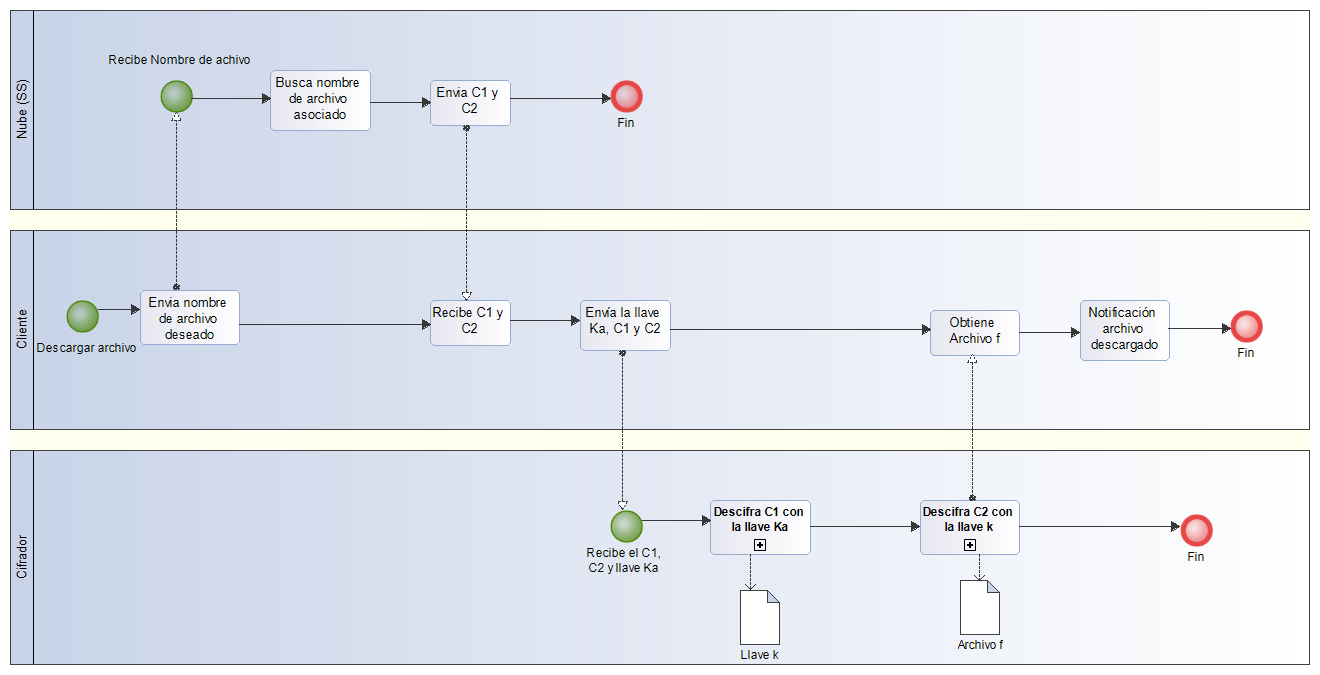
\includegraphics[width=16cm, height=7cm]{./images/bp_descargar.png}
	\caption{BPMN Subir archivo.}

\end{figure}

\begin{figure}[H]
\centering
	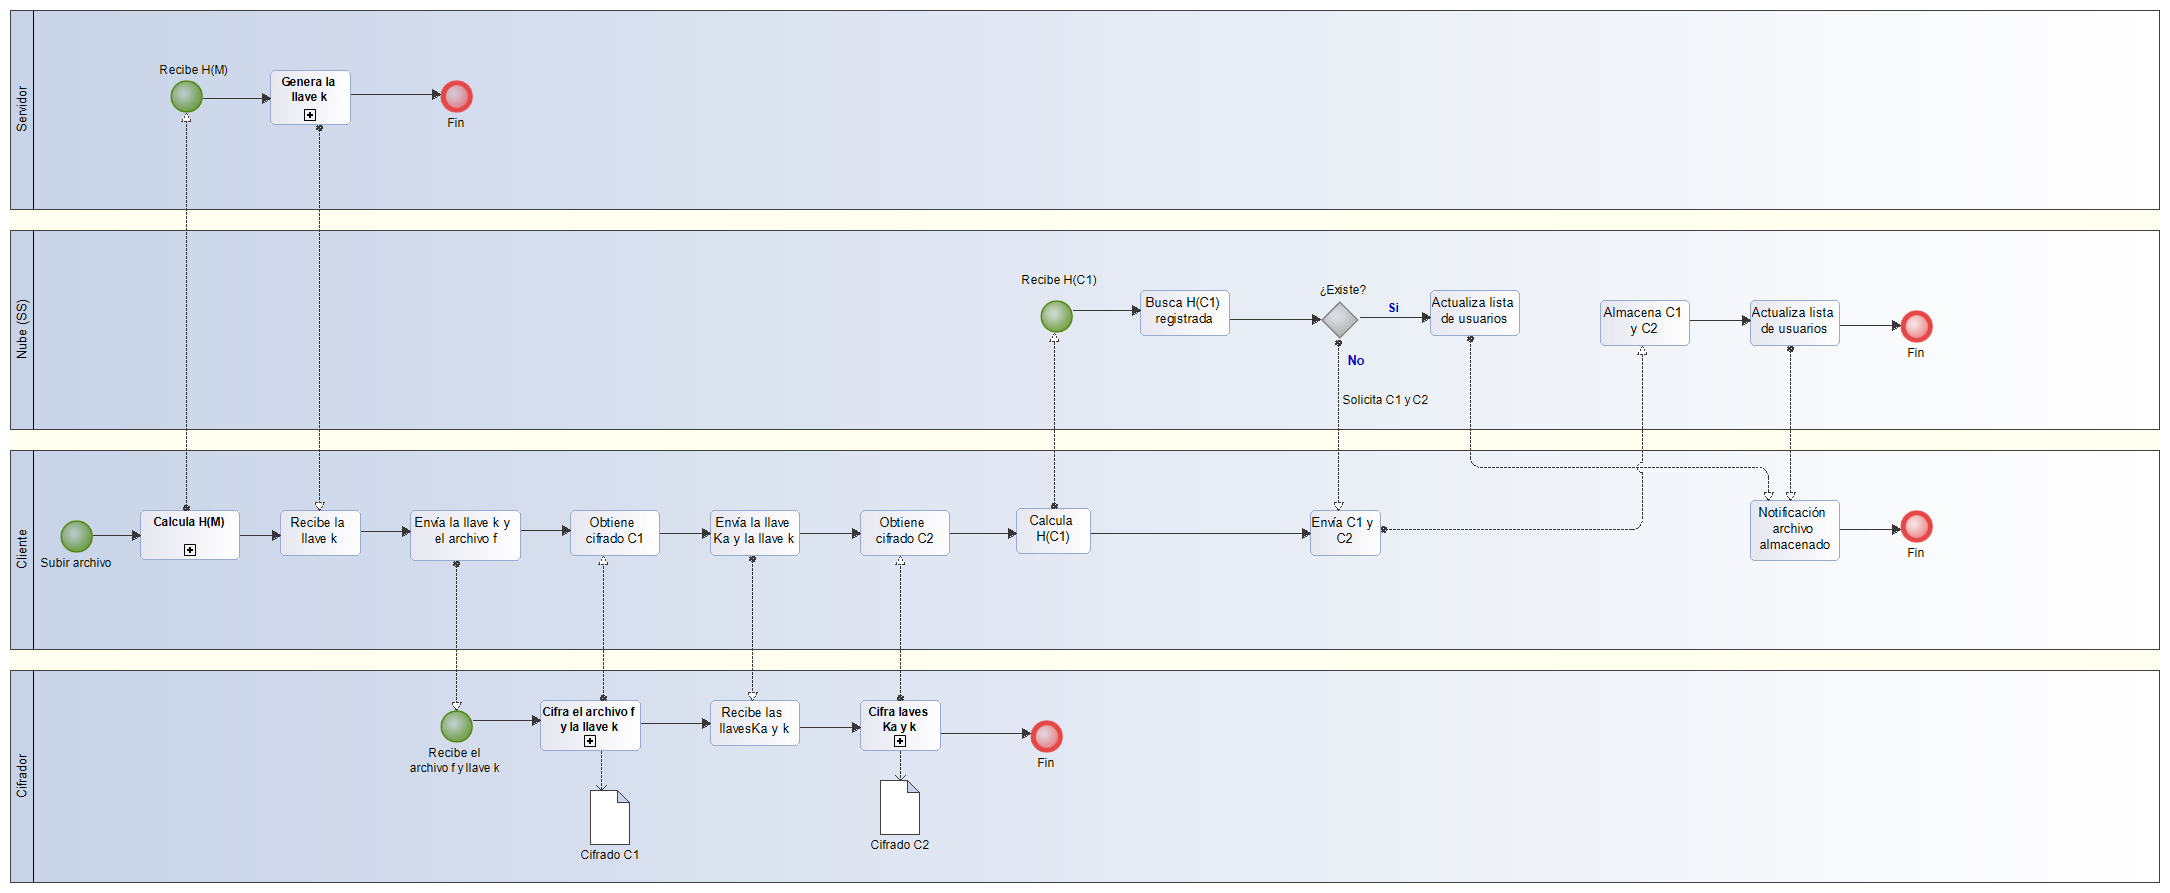
\includegraphics[width=16cm, height=7cm]{./images/bp_subir.png}
	\caption{BPMN Descargar archivo.}

\end{figure}

\section{Requerimientos Funcionales. }

\begin{table}[htb]
\centering
\begin{tabular}{| p{2cm} |  p{13.5cm} |}
\hline
\multicolumn{2}{|c|}{\textbf{Servidor de Llaves}} \\ \hline
\textbf{ID} &  \textbf{Descripción} \\
\hline \hline
RF – SLL1 & El sistema permitirá la generación de llaves de usuario a través de una clave secreta (Kg) propia del servidor de llaves. \\ \hline
%RF – SLL2 & El sistema debe gestionar 3 estados en el servidor de llaves: Generación, Cambios y Eliminación de llaves de usuarios para manipular un archivo. \\ \hline
%RF – SLL3 & El sistema comenzará la creación de una llave (K) cuando el usuario solicite la carga de un archivo a almacenar. \\ \hline
%RF – SLL4 & El sistema deberá enviar al cliente la llave generada en el servidor de llaves (K) del archivo que el usuario solicitó carga al servicio de almacenamiento. \\ \hline
RF – SLL2 & El sistema permitirá la firma a ciegas (y) de cualquier archivo que se desee almacenar. \\ \hline
%RF – SLL3 & El sistema actualizará la base de datos del servidor de llaves cada vez que una nueva firma (y) sea generada dentro de éste. \\ \hline
%RF – SLL7 & El sistema detectará mediante la función hash del archivo [H(F)] si se le ha generado anteriormente una llave (K), si ésta existe en la base de datos se procederá a enviarla al usuario que la solicita. \\ \hline
%RF – SLL8 & El sistema modificará la llave (K) para un archivo cuando este sea modificado por el propietario del archivo (F). \\ \hline
%RF – SLL9 & El sistema eliminará la llave (K) para un archivo cuando este sea eliminado del servicio de almacenamiento por el usuario. \\ \hline
\end{tabular}
\caption{Requerimientos funcionales del servidor de llaves}
\label{Servidor de Llaves }
\end{table}


\begin{table}[htb]
\centering
\begin{tabular}{| p{2cm} |  p{13.5cm} |}
\hline
\multicolumn{2}{|c|}{\textbf{Cliente}} \\ \hline
\textbf{ID} &  \textbf{Descripción} \\
\hline \hline
RF – CL1 & El sistema permitirá al usuario gestionar archivos: Subir, Descargar, Eliminar \\ \hline
%RF – CL2 & El sistema permitirá al usuario calcular a su archivo (F) una función hash [H(F)] cuando dicho usuario solicite una nueva carga de éste. \\ \hline
RF – CL2 & El sistema permitirá al usuario subir un archivo (F) cifrado al servicio de almacenamiento  \\ \hline
%RF – CL4 & El sistema entregará al cliente la llave (K) generada en el servidor de llaves del archivo (F) que el usuario solicitó cargar al servicio de almacenamiento.  \\ \hline
%RF – CL5 & El sistema mandará a cifrar la llave (K) obtenida del servidor de llaves junto con el archivo (F) que el usuario desea cargar al servicio de almacenamiento. \\ \hline
%RF – CL6 & El sistema obtendrá el cifrado C1 correspondiente al archivo original (F)  y lo mandará al cliente, cifrado que el usuario cargará al servicio de almacenamiento.  \\ \hline
%RF – CL7  & El sistema calculará al cifrado C1 una función hash [H(C1)] \\ \hline
%RF – CL8  & El sistema mandará a cifrar la llave secreta (Ka) del usuario junto con la llave (K) obtenida del servidor de llaves del archivo (F) que éste usuario desea cargar al servicio de almacenamiento. \\ \hline
%RF – CL9  & El sistema obtendrá el cifrado C2 correspondiente a la llave secreta (Ka) del usuario y lo mandará al cliente, cifrado que el usuario cargará al servicio de almacenamiento. \\ \hline
%RF – CL10 & El sistema enviará [H(C1)] hacia el servicio de almacenamiento para su evaluación. \\ \hline
RF – CL3 & El sistema permitirá al usuario descargar un archivo (F) descifrado elejido de su lista de archivos en el servicio de almacenamiento\\ \hline
%RF – CL12 & El sistema notificará al usuario el estatus final de la gestión de sus archivos en el servicio de almacenamiento.  \\ \hline
RF – CL4 &El sistema permitirá al usuario eliminar un archivo (F) cuando el usuario elige alguno de su lista de archivos cargados en el servicio de almacenamiento  \\ \hline
%RF – CL14 & El sistema entregará al cliente el cifrado C1 correspondiente al archivo (F) que el usuario eligió y el cifrado C2 que corresponde a la llave (K) del mismo archivo. \\ \hline
%RF – CL15 & El sistema enviará desde el cliente al módulo cifrador la llave secreta (Ka) del usuario junto con el cifrado C1 y C2.  \\ \hline
%RF – CL16 & El sistema obtendrá el archivo original (F) que solicitó el usuario para la descarga.  \\ \hline
RF – CL5 & El sistema generará la llave (K) correspondiente a la firma (Y) que envió el servidor de llaves  \\ \hline
%RF – CL18 & El sistema enviará al servidor de almacenamiento el nombre del archivo (F) que el usuario solicite eliminar.  \\ \hline
%RF – MC1 & El sistema recibirá en el modulo cifrador la llave (K) obtenida del servidor de llaves junto con el archivo (F) que el usuario desea cargar. \\ \hline
RF – CL6 & El sistema cifrará el archivo (F) que el usuario a solicitado \\ \hline
%RF – MC3 & El sistema enviará al cliente el archivo C1 obtenido en el módulo cifrador. \\ \hline
%RF – MC4 & El sistema recibirá en el módulo cifrador la llave secreta (Ka) del usuario junto con la llave (K) obtenida del servidor de llaves del archivo (F) que éste usuario desea cargar \\ \hline
RF – CL7 & El sistema descifrará el archivo (F) que el usuario a solicitado  \\ \hline
%RF – MC6 & El sistema enviará al cliente el archivo C2 obtenido en el módulo cifrador. \\ \hline
%RF – MC7 & El sistema recibirá en el modulo cifrador la llave secreta (Ka) junto con el cifrado C1 y el cifrado C2 que el usuario solicite descargar.\\ \hline
%RF – MC9 & El sistema descifrará el C2 junto con la llave (K) que el usuario a solicitado descargar y generará el archivo original (F).\\ \hline
\end{tabular}
\caption{Requerimientos funcionales del cliente}
\label{Cliente }
\end{table}


\begin{table}[htb]
\centering
\begin{tabular}{| p{2cm} |  p{13.5cm} |}
\hline
\multicolumn{2}{|c|}{\textbf{Servicio de almacenamiento (Nube)}} \\ \hline
\textbf{ID} &  \textbf{Descripción} \\
\hline \hline
RF – SA1 & El sistema permitirá al servicio de almacenamiento gestionar archivos: Almacenar, Descargar y Eliminar.\\ \hline
%RF – SA2 & El sistema creará una base de datos con los cifrados que cada usuario tenga registrados dentro del servicio de almacenamiento.\\ \hline
RF – SA2 & El sistema permitirá al servicio de almacenamiento guardar cualquier cifrado que el usuario solicite cargar. \\ \hline
RF – SA3 & El sistema permitirá al servicio de almacenamiento descargar cualquier cifrado que el usuario tenga en su lista de archivos. \\ \hline
RF – SA4 & El sistema permitirá al servicio de almacenamiento eliminar cualquier cifrado que el usuario tenga en su lista de archivos. \\ \hline
%RF – SA6 & El sistema actualizará dentro de la base de datos del servicio de almacenamiento, la lista de archivos (F) que el usuario a gestionado dentro de éste. \\ \hline
%RF – SA7 & El sistema entregará [H(C1)] generado por el cliente al servicio de almacenamiento \\ \hline
%RF – SA8 & El sistema almacenará en una base de datos dentro del servicio de almacenamiento a [H(C1)] asociando al cliente que lo envió. \\ \hline
%RF – SA9 & El sistema corroborará la existencia [H(C1)] dentro de la base de datos, si existe procederá al RF – SA6,  si no procederá al RF – SA3\\ \hline
%RF – SA10 & El sistema entregará al servidor de almacenamiento el nombre del archivo (F) que el usuario solicite eliminar.\\ \hline
%RF – SA11 & El sistema eliminará el nombre del archivo (F) de la lista de archivos que el usuario tiene registrados en la base de datos del servidor de almacenamiento. \\ \hline
%RF – SA12 & El sistema enviará una notificación al cliente con el estatus de cada gestión hecha por el usuario sobre sus archivos. \\ \hline
%RF – SA13 & El sistema recibirá el nombre del archivo (F) que el usuario solicita descargar.\\ \hline
%RF – SA14 & El sistema buscará el nombre del archivo (F) en la base de datos de los cifrados que tiene el usuario registrados en el servicio de almacenamiento.\\ \hline
%RF – SA15 & El sistema enviará al cliente el archivo C1 correspondiente al archivo (F) que el usuario eligió y el cifrado C2 que corresponde a la llave (K) del mismo archivo. \\ \hline
\end{tabular}
\caption{Requerimientos funcionales del Servicio de almacenamiento (Nube)}
\label{Servicio de almacenamiento (Nube) }
\end{table}


\section{Requerimientos No Funcionales }
\begin{longtable}{| p{1.5cm} | p{3cm} | p{11cm} |}

% aquí añadimos el encabezado de la primera hoja.
\hline
\multicolumn{3}{|c|}{\textbf{Requerimientos No Funcionales}} \\ \hline
\textbf{ID} &  \textbf{Atributo} & \textbf{Descripción}\\
\hline \hline
\endfirsthead

% aquí añadimos el encabezado del resto de hojas.
\hline
\textbf{ID} &  \textbf{Atributo} & \textbf{Descripción}\\
\hline \hline
\endhead

% aquí añadimos el fondo de todas las hojas, excepto de la última.
\multicolumn{3}{|c|}{Sigue en la página siguiente.}
\endfoot

% aquí añadimos el fondo de la última hoja.
\endlastfoot

% aquí añadimos el cuerpo de la tabla.
RNF1 & Eficiencia &  \begin{itemize} 
   \item El servidor de llaves tendrá la capacidad de realizar 1000 peticiones de gestión de almacenamiento de archivos por segundo. 
   \item El sistema podrá funcionar de forma correcta con usuarios conectados de manera concurrente. 
   \item Los archivos que sean gestionados dentro del servidor de almacenamiento, deben ser actualizados en la base datos y la visualización de cada cliente de manera casi inmediata. 
  \end{itemize}
\\ \hline

RNF2 & Fiabilidad &  \begin{itemize} 
  \item La pérdida de consultas en el servidor de llaves es menor a 3 veces el máximo de consultas realizadas. 
   \item Los archivos almacenados en el servidor de almacenamiento deben ser recuperados por el usuario al instante en que este lo solicite. 
   \item El tiempo de latencia que existe entre el servidor de llaves y el cleinte será de máximo 118ms. 
 \end{itemize}
\\ \hline

RNF3 & Seguridad & \begin{itemize} 
    \item El sistema almacenará los datos de los usuarios y sus contraseñas en una base de datos MySQL, dichos datos serán modificados mínimo 2  veces al año.  
   \item Se autenticarán los clientes antes de comenzar el proceso de generación de llaves de archivo. 
   \item El servidor de llaves firmará claves para un sólo mensaje a la vez sin saber el contenido de éste. 
   \item El inicio de sesión de usuarios estará protegido en un canal seguro utilizando almoritmos criptográficos. 
   \item Las funciones hash de archivos a almacenar utilizarán la función criptográfica SHA-(256)
 \end{itemize}

\\ \hline 
RNF4 & Mantenibilidad & \begin{itemize}
   \item Cuaquier nuevo requerimiento funcional o no funcional tendrá que ser analizado y diseñado para poder cuantificar las implicaciones que este tendrá sobre el funcionamiento del sistema. 
   \item El sistema contará con un plan de pruebas que facilitará la identificación de posibles fallas existentes en el funcionamiento de este. 
 \end{itemize}
\\ \hline
\caption{Requerimientos no funcionales del sistema}
\label{Servidor de Llaves }
\end{longtable}




\section{Descripción General del Desarrollo del Protocolo}
El protocolo criptográfico para evitar duplicados almacenados en la nube, es un proyecto que involucra la tecnología de software para ofrecer un funcionamiento eficiente y útil para las necesidades de los usuarios que se encuentran inmersos en el cómputo nube. 
Nuestro protocolo, se compone a su vez de diferentes módulos. Cada uno de ellos busca satisfacer: \\ 

\begin{itemize}

\item La seguridad de los archivos de los usuarios en la nube
\item Almacenamiento seguro en la sube
\item Conexión de diversos usuarios 
\item Ahorro en el consumo de espacio ofrecido en la nube 
\item Fácil acceso al almacenamiento de los archivos de los usuarios 

\end{itemize} 

Para lograrlo, el protocolo criptográfico se compone de diversos módulos que a su vez integran diferentes aplicaciones criptográficas. Dichos módulos serán detallados en las próximas secciones. 

\section{Aplicación Criptográfica (Cifrado / Descifrado)}

Éste módulo del protocolo es de suma importancia para ofrecer la seguridad de los archivos como se menciona anteriormente, ya que en éste módulo se lleva a cabo para blindar un archivo, es decir cifrarlo.  En este módulo participan: 

	\begin{itemize}
	\item El archivo que se almacenará en la nube.
	\item La clave para poder cifrarlo, que en este caso es la llave \textit{(z)} generada por el cliente en el módulo anterior. 
	\end{itemize}
El desarrollo de éste módulo, fue realizado como el módulo anterior en el lenguaje de programación Python versión 2.7.3. Además de que para la implementación del algoritmo de cifrado AES se utilizó principalmente la biblioteca criptográfica Pycripto 2.3. 

\subsection{Cifrado}
Éste algoritmo que forma parte de la aplicación criptográfica, se lleva a cabo del lado del cliente, dicho algoritmo de cifrado se encargará de brindar la seguridad a los archivos que los usuarios deseen almacenar en la nube. \\
El cifrado de archivos se lleva a cabo bajo la utilización del algoritmo de cifrado \textbf{AES} que proveé la librería criptográfica \textbf{PyCripto 2.3} propia del lenguaje \textbf{Python}. Ésta libreria poseé la seguridad necesaria para satisfacer a los requerimientos del protocolo criptográfico.  \\ 
La implementación del algoritmo, se llevó a cabo de la siguiente manera: 

	\begin{itemize}
		\item Las librerías utilizadas para llevar a cabo el cifrado de archivos son las siguientes
			\begin{figure}[H]
			\centering
			\includegraphics[width=10cm, height=1.5cm]{./images/cifrado/01.jpg}
			\caption{Librerías de Python (Cifrado)}
			\label{fig:6-2-1} 
			\end{figure} 
		Siendo \textbf{haslib, Crypto.Cipher.AES, Crypto.Util.Counter, hmac} librerías criptográficas, es decir, utilizadas para llevar a cabo operaciones relacionadas con la implementación del algoritmo de cifrado \textit{AES} en sus 3 tipos de tamaños de claves \textit{(128, 192, 256 bits)}.\\ \\ 
La librería \textbf{tkFileDialog} utilizada para cuando el usuario desee elegir desde su PC un archivo para almacenarlo en la nube, se abra un panel de archivos, permitiendo acceder a sus carpetas personales, y de manera gráfica, dicho usuario pueda elegir el archivo con solo darle un clic. \\ \\ 
\textbf{Base 64} Una librería utilizada para convertir las salidas del algoritmo \textit{AES} a caracteres dentro del \textit{código ASCII}, ya que \textit{AES} involucra funciones que obtienen a la salida caracteres en el sistema hexadecimal y son difíciles de procesar en su forma original para su uso posterior. 


		\item Para poder comenzar el proceso de cifrado, es necesario obtener la clave que se utilizará para llevar a cabo el proceso. \\ Dicha clave se obtiene de la siguiente manera: 
			\begin{figure}[H]
			\centering
			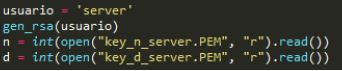
\includegraphics[width=10cm, height=1cm]{./images/cifrado/02.jpg}
			\caption{Obtención de Clave de Cifrado}
			\label{fig:6-2-2} 
			\end{figure} 
	Abrimos el archivo \textbf{key\_z} y almacenamos su contenido en la variable \textbf{contentK}. Éste archivo contiene la clave que se necesita para poder cifrar el archivo que el usuario desea, dicha \textit{clave (z)} fue generada y escrita en este archivo en el módulo anterior. 

		\item Se crea un objeto de tipo \textit{AES} que almacenamos en la variable \textbf{cipher}, el cual contiene como parámetros la clave que obtuvo del archivo  \textbf{key\_z}, el modo de operación que se utilizará \textbf{(CTR)}, etc.
			\begin{figure}[H]
			\centering
			
\includegraphics[width=15cm, height=1cm]{./images/cifrado/03.jpg}
			\caption{Objeto de Tipo AES}
			\label{fig:6-2-3} 
			\end{figure} 

		\item Para cifrar el archivo, mandamos llamar al método \textbf{\textit{encrypt(m)}} \textit{(m almacena el contenido del archivo que se desea cifrar)} y almacenamos el resultado de dicho método en la variable \textbf{ctext.}
			\begin{figure}[H]
			\centering
			
\includegraphics[width=10cm, height=1cm]{./images/cifrado/04.jpg}
			\caption{Método Encrypt}
			\label{fig:6-2-4} 
			\end{figure} 

		\item Para finalizar, mandamos escribir a un archivo temporal el cifrado que obtuvimos en la variable \textbf{ctext.}
			\begin{figure}[H]
			\centering
			\includegraphics[width=13cm, height=1.5cm]{./images/cifrado/05.jpg}
			\caption{Escribir Cifrado en Archivo Temporal}
			\label{fig:6-2-4} 
			\end{figure} 


	\end{itemize}


\subsection{Descifrado}
Éste algoritmo que forma parte de la aplicación criptográfica, al igual que el cifrado, se lleva a cabo del lado del cliente, éste algoritmo será el encargado de que los usuarios puedan recuperar sus archivos originales, es decir, tomar de la nube aquel archivo que se encuentre cifrado y posteriormente descifrarlo para poder acceder a este archivo en su forma original. \\
El descifrado de archivos se lleva a cabo bajo la utilización del algoritmo de descifrado \textbf{AES} que, al igual que el cifrado lo proveé la librería criptográfica \textbf{PyCripto 2.3} propia del lenguaje \textbf{Python}.   \\ 
La implementación del algoritmo, se llevó a cabo de la siguiente manera: 

\begin{itemize}
	\item Las librerías utilizadas para llevar a cabo el descifrado de archivos son las siguientes: 
			\begin{figure}[H]
			\centering
			\includegraphics[width=8.5cm, height=1cm]{./images/descifrado/01.jpg}
			\caption{Librerías de Python (Descifrado)}
			\label{fig:6-3-1} 
			\end{figure} 
Siendo \textbf{Crypto.Cipher.AES, Crypto.Util.Counter}, librerías criptográficas, es decir, utilizadas para llevar a cabo operaciones relacionadas con la implementación del algoritmo de descifrado \textit{AES} en sus 3 tipos de tamaños de claves \textit{(128, 192, 256 bits)}. 

	\item Al igual que en el proceso de cifrado, para comenzar dicho proceso es necesario obtener la clave que se utilizará para el descifrado. Dicha clave se obtiene de la siguiente manera:  

			\begin{figure}[H]
			\centering
			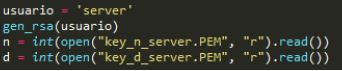
\includegraphics[width=10cm, height=1cm]{./images/cifrado/02.jpg}
			\caption{Obtención de Clave de Descifrado}
			\label{fig:6-3-2} 
			\end{figure} 

Abrimos el archivo \textbf{key\_z} y almacenamos su contenido en la variable \textbf{contentK}. 

		\item El siguiente paso, es abrir el archivo temporal que se generó al momento de cifrar el archivo del usuario. 
			\begin{figure}[H]
			\centering
			
\includegraphics[width=10cm, height=1cm]{./images/descifrado/03.jpg}
			\caption{Obtención del cifrado}
			\label{fig:6-3-3} 
			\end{figure} 

Una vez dentro del archivo, almacenamos el cifrado en la variable \textbf{textcifrado} para utilizarlo posteriormente. 

		\item Creamos un objeto \textit{AES} que almacenamos en la variable \textbf{ciphe}r, el cual contiene como parámetros la llave que obtuvo del archivo \textbf{key\_z }, el modo de operación que se utilizará para el descifrado\textbf{(CTR)}, etc.
			\begin{figure}[H]
			\centering
			
\includegraphics[width=15cm, height=1cm]{./images/cifrado/03.jpg}
			\caption{Objeto de Tipo AES}
			\label{fig:6-3-4} 
			\end{figure} 


		\item Desciframos el archivo, mandamos llamar al método \textbf{\textit{decrypt(textcifrado)}}  y almacenamos el resultado de dicho método en la variable \textbf{plaintext}
			\begin{figure}[H]
			\centering
			\includegraphics[width=9cm, height=1cm]{./images/descifrado/05.jpg}
			\caption{Método Decrypt}
			\label{fig:6-3-5} 
			\end{figure} 

		\item Para finalizar, mandamos escribir a un archivo \textbf{fname} \textit{(Es el nombre del archivo original del usuario)} el archivo tal y como estaba antes de cifrarlo. 
			\begin{figure}[H]
			\centering
			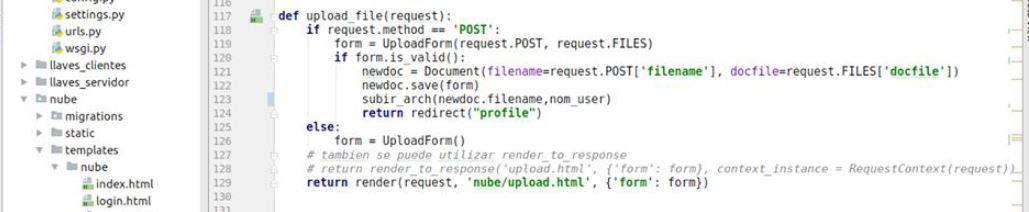
\includegraphics[width=10cm, height=1.5cm]{./images/descifrado/06.jpg}
			\caption{Escribir Archivo Original en la Ruta Inicial}
			\label{fig:6-3-6} 
			\end{figure} 

\end{itemize}






\chapter{Conclusiones y Trabajo a Futuro}
\section{Conclusiones}



\appendix
\chapter{Código fuente del prototipo 2}


\backmatter
\addcontentsline{toc}{chapter}{Bibliograf\'ia}
\bibliographystyle{abbrv} %{plain}
\bibliography{bibliografia}
\end{document}

